\documentclass[12pt, a4paper, twoside]{report}
%%% Nyomtatásnál Figyelni a kétoldalasságra és a kötésre!!!
\setcounter{tocdepth}{3}
\setcounter{secnumdepth}{3}
\newcounter{para}
\newcommand\mypara{\par\refstepcounter{para}\thepara\space}
\usepackage{verbatim}
\usepackage[T1]{fontenc}
\usepackage[utf8]{inputenc}
%\usepackage[UTF8]{ctex}     %% kínai karakterekhez
\usepackage{anysize}
\usepackage[left=4cm,top=3cm, bottom=3cm, right=3cm]{geometry}
%\usepackage{cite}
%\usepackage[square,numbers]{natbib}
%\bibliographystyle{abbrvnat}

%\usepackage{xcolor}
\usepackage[table,xcdraw,dvipsnames]{xcolor}
\colorlet{RED}{red}
\usepackage{amsmath}
\usepackage{mathtools}
\newcommand{\norm}[1]{\left\lVert#1\right\rVert}
\usepackage{amssymb}
\usepackage{eurosym}
\usepackage{graphics}
\usepackage{graphicx} %===!!!=== Ezt én adtam hozzá
\usepackage{caption} %===!!!=== Ezt én adtam hozzá
\usepackage{subcaption} %===!!!=== Ezt én adtam hozzá
%\usepackage{subfig}
%\usepackage{subfigure}
\usepackage{tikz}
\usepackage{pgfplots}
\pgfplotsset{compat=1.9}
\usepackage{pgfkeys}
\usepgfplotslibrary{polar}
\usetikzlibrary{patterns}
\usepackage{pgfpages}
\usepackage{soul}
%\usepackage{algorithm}
\usepackage{algpseudocode}
\makeatletter
\def\BState{\State\hskip-\ALG@thistlm}
\makeatother

\usepackage{xcolor} % changed from \usepackage{xcolor}
%\usepackage[dvipsnames]{xcolor}
\usepackage{gensymb}
\usepackage{setspace}
\usepackage{circuitikz}
\usepackage{indentfirst}
\usepackage{pgfplotstable}
\usepackage{siunitx}
%\usepackage{subfigure}
\usepackage{fancyhdr}
\usepackage{multirow}
\pagestyle{fancy}
\fancyhead{}
\fancyhead[RO]{\textsl{\rightmark}}
\fancyhead[LE]{\textsl{\leftmark}}
%\usetikzlibrary{external}
%\tikzexternalize % activate!
\usepackage{breqn}
\usepackage[absolute,overlay]{textpos}
\usepackage{transparent}
\usepackage{eso-pic}
\usetikzlibrary{calc}
\usepackage{lscape}
\usetikzlibrary{circuits.logic.US,circuits.logic.IEC}
\usepackage{multirow}
\usepackage{hhline}
\usepackage{textpos}

%% Saját package-ek
\usepackage{textcomp}
\usepackage{mfirstuc}
\usepackage{longtable}
\usepackage{textcomp}
\usepackage{tabu}
\usepackage[shortlabels]{enumitem}
\usepackage{arydshln}
\setlength{\dashlinedash}{0.2pt}
\setlength{\dashlinegap}{4.5pt}
\setlength{\arrayrulewidth}{0.2pt}
\usepackage{tabularx}
\usepackage{ltablex}\keepXColumns
\usepackage{adjustbox}
\usepackage[ruled,vlined]{algorithm2e}
%\usepackage{hyperref}
\usepackage{enumitem}
\newlist{inparaenum}{enumerate}{2}% allow two levels of nesting in an enumerate-like environment
\setlist[inparaenum]{nosep}% compact spacing for all nesting levels
\setlist[inparaenum,1]{label=\bfseries\roman*.}% labels for top level
\setlist[inparaenum,2]{label=\roman{inparaenumi}\emph{\alph*})}% labels for second level

\usepackage[backend=bibtex, style=ieee, sorting=none, defernumbers=true, url=false, doi=false]{biblatex} %%% true/fals be és kikapcsolás!!
\addbibresource{dolgozat} %bib fájl
% use boldface for specific author in biblatex bibliography
% http://tex.stackexchange.com/questions/73136/make-specific-author-bold-using-biblatex
%
% usage:
% % use boldface for specific author in biblatex bibliography
% http://tex.stackexchange.com/questions/73136/make-specific-author-bold-using-biblatex
%
% usage:
% % use boldface for specific author in biblatex bibliography
% http://tex.stackexchange.com/questions/73136/make-specific-author-bold-using-biblatex
%
% usage:
% \input{boldauthorname}
% ...
% \begin{document}
% \boldname{Doe}{John}{J.}
% \printbibliography
% \end{document}
%
% deactivate:
% \boldname{}{}{}
%
\def\makenamesetup{%
  \def\bibnamedelima{~}%
  \def\bibnamedelimb{ }%
  \def\bibnamedelimc{ }%
  \def\bibnamedelimd{ }%
  \def\bibnamedelimi{ }%
  \def\bibinitperiod{.}%
  \def\bibinitdelim{~}%
  \def\bibinithyphendelim{.-}}
\newcommand*{\makename}[2]{\begingroup\makenamesetup\xdef#1{#2}\endgroup}

\newcommand*{\boldname}[3]{%
  \def\lastname{#1}%
  \def\firstname{#2}%
  \def\firstinit{#3}}
\boldname{}{}{} %% több keresztnév esetén nem space kell hanem ~ karakter !!!!

% Patch new definitions
%%%%%%%%%%%%%%%%%% saját módosított változat %%%%%%%%%%%%%%%%%%%%%%
\renewcommand{\mkbibnamegiven}[1]{%
  \makename{\currfname}{#1}%
  \makename{\findfname}{\firstname}%
  \makename{\findinit}{\firstinit}%
  \ifboolexpr{ test {\ifdefequal{\currfname}{\findfname}} or test {\ifdefequal{\currfname}{\findinit}} }%
    {\kern-0.4em}
    {\kern-0.4em}%
}

\renewcommand{\mkbibnamefamily}[1]{%
  \makename{\currlname}{#1}%
  \makename{\findlname}{\lastname}%
  \ifboolexpr{ test {\ifdefequal{\currlname}{\findlname}} }%
    {\ifboolexpr{ test {\ifdefequal{\currfname}{\findfname}} or test {\ifdefequal{\currfname}{\findinit}} }
        {\mkbibbold{\currfname~\currlname}}
        {\currfname~\currlname}
    }
    {\currfname~\currlname}%
} 

%%%%%%%%%%%%%%%%%%%%%% eredeti ez volt %%%%%%%%%%%%%%%%%%%%
%\renewcommand{\mkbibnamegiven}[1]{%
%  \makename{\currname}{#1}%
%  \makename{\findname}{\firstname}%
%  \makename{\findinit}{\firstinit}%
%  \ifboolexpr{ test {\ifdefequal{\currname}{\findname}}%
%    or test {\ifdefequal{\currname}{\findinit}} }%
%  {\mkbibbold{#1}}{#1}%
%}
%
%\renewcommand{\mkbibnamefamily}[1]{%
%  \makename{\currname}{#1}%
%  \makename{\findname}{\lastname}%
%  \ifboolexpr{ test {\ifdefequal{\currname}{\findname}} }%
%  {\mkbibbold{#1}}{#1}%
%}


% ...
% \begin{document}
% \boldname{Doe}{John}{J.}
% \printbibliography
% \end{document}
%
% deactivate:
% \boldname{}{}{}
%
\def\makenamesetup{%
  \def\bibnamedelima{~}%
  \def\bibnamedelimb{ }%
  \def\bibnamedelimc{ }%
  \def\bibnamedelimd{ }%
  \def\bibnamedelimi{ }%
  \def\bibinitperiod{.}%
  \def\bibinitdelim{~}%
  \def\bibinithyphendelim{.-}}
\newcommand*{\makename}[2]{\begingroup\makenamesetup\xdef#1{#2}\endgroup}

\newcommand*{\boldname}[3]{%
  \def\lastname{#1}%
  \def\firstname{#2}%
  \def\firstinit{#3}}
\boldname{}{}{} %% több keresztnév esetén nem space kell hanem ~ karakter !!!!

% Patch new definitions
%%%%%%%%%%%%%%%%%% saját módosított változat %%%%%%%%%%%%%%%%%%%%%%
\renewcommand{\mkbibnamegiven}[1]{%
  \makename{\currfname}{#1}%
  \makename{\findfname}{\firstname}%
  \makename{\findinit}{\firstinit}%
  \ifboolexpr{ test {\ifdefequal{\currfname}{\findfname}} or test {\ifdefequal{\currfname}{\findinit}} }%
    {\kern-0.4em}
    {\kern-0.4em}%
}

\renewcommand{\mkbibnamefamily}[1]{%
  \makename{\currlname}{#1}%
  \makename{\findlname}{\lastname}%
  \ifboolexpr{ test {\ifdefequal{\currlname}{\findlname}} }%
    {\ifboolexpr{ test {\ifdefequal{\currfname}{\findfname}} or test {\ifdefequal{\currfname}{\findinit}} }
        {\mkbibbold{\currfname~\currlname}}
        {\currfname~\currlname}
    }
    {\currfname~\currlname}%
} 

%%%%%%%%%%%%%%%%%%%%%% eredeti ez volt %%%%%%%%%%%%%%%%%%%%
%\renewcommand{\mkbibnamegiven}[1]{%
%  \makename{\currname}{#1}%
%  \makename{\findname}{\firstname}%
%  \makename{\findinit}{\firstinit}%
%  \ifboolexpr{ test {\ifdefequal{\currname}{\findname}}%
%    or test {\ifdefequal{\currname}{\findinit}} }%
%  {\mkbibbold{#1}}{#1}%
%}
%
%\renewcommand{\mkbibnamefamily}[1]{%
%  \makename{\currname}{#1}%
%  \makename{\findname}{\lastname}%
%  \ifboolexpr{ test {\ifdefequal{\currname}{\findname}} }%
%  {\mkbibbold{#1}}{#1}%
%}


% ...
% \begin{document}
% \boldname{Doe}{John}{J.}
% \printbibliography
% \end{document}
%
% deactivate:
% \boldname{}{}{}
%
\def\makenamesetup{%
  \def\bibnamedelima{~}%
  \def\bibnamedelimb{ }%
  \def\bibnamedelimc{ }%
  \def\bibnamedelimd{ }%
  \def\bibnamedelimi{ }%
  \def\bibinitperiod{.}%
  \def\bibinitdelim{~}%
  \def\bibinithyphendelim{.-}}
\newcommand*{\makename}[2]{\begingroup\makenamesetup\xdef#1{#2}\endgroup}

\newcommand*{\boldname}[3]{%
  \def\lastname{#1}%
  \def\firstname{#2}%
  \def\firstinit{#3}}
\boldname{}{}{} %% több keresztnév esetén nem space kell hanem ~ karakter !!!!

% Patch new definitions
%%%%%%%%%%%%%%%%%% saját módosított változat %%%%%%%%%%%%%%%%%%%%%%
\renewcommand{\mkbibnamegiven}[1]{%
  \makename{\currfname}{#1}%
  \makename{\findfname}{\firstname}%
  \makename{\findinit}{\firstinit}%
  \ifboolexpr{ test {\ifdefequal{\currfname}{\findfname}} or test {\ifdefequal{\currfname}{\findinit}} }%
    {\kern-0.4em}
    {\kern-0.4em}%
}

\renewcommand{\mkbibnamefamily}[1]{%
  \makename{\currlname}{#1}%
  \makename{\findlname}{\lastname}%
  \ifboolexpr{ test {\ifdefequal{\currlname}{\findlname}} }%
    {\ifboolexpr{ test {\ifdefequal{\currfname}{\findfname}} or test {\ifdefequal{\currfname}{\findinit}} }
        {\mkbibbold{\currfname~\currlname}}
        {\currfname~\currlname}
    }
    {\currfname~\currlname}%
} 

%%%%%%%%%%%%%%%%%%%%%% eredeti ez volt %%%%%%%%%%%%%%%%%%%%
%\renewcommand{\mkbibnamegiven}[1]{%
%  \makename{\currname}{#1}%
%  \makename{\findname}{\firstname}%
%  \makename{\findinit}{\firstinit}%
%  \ifboolexpr{ test {\ifdefequal{\currname}{\findname}}%
%    or test {\ifdefequal{\currname}{\findinit}} }%
%  {\mkbibbold{#1}}{#1}%
%}
%
%\renewcommand{\mkbibnamefamily}[1]{%
%  \makename{\currname}{#1}%
%  \makename{\findname}{\lastname}%
%  \ifboolexpr{ test {\ifdefequal{\currname}{\findname}} }%
%  {\mkbibbold{#1}}{#1}%
%}


\usepackage{sectsty}

%\usepackage{ulem}
%\newcommand{\soutthick}[1]{%
%    \renewcommand{\ULthickness}{2.4pt}%
%       \sout{#1}%
%    \renewcommand{\ULthickness}{.4pt}% Resetting to ulem default
% \usepackage{MnSymbol,wasysym}
%\DeclareSourcemap{
  %\maps[datatype=bibtex]{
    %\map{
      %\step[fieldsource=issue, match=\regexp{\A(\d+)\Z}, final]
      %\step[fieldset=number, fieldvalue={$1}]
      %\step[fieldset=issue, null]
    %}
  %}
%}

\newcommand{\myparagraph}[1]{\paragraph{#1}\mbox{}\\}


\def\myuni{Universiy of Pannonia}
\def\myfaculty{Faculty of Information Technology}
\def\myschool{Doctoral School of Information Science}
\def\mytitle{Optimal Current Control for Domestic Power converters}
\def\myauthor{L\'aszl\'o Rich\'ard Neukirchner}
\def\mydate{2021}
\def\mysupervisor{dr. Attila Magyar}


%\rhead{L\'aszlo Richard Neukirchner (ZOK4EW) 2014/20}
\renewcommand{\contentsname}{List of contents}
\renewcommand{\figurename}{Figure}
\renewcommand{\tablename}{Table}
\renewcommand{\chaptername}{Chapter}
\renewcommand{\bibname}{Bibliography}
\let\oldref\ref
\renewcommand{\ref}[1]{(\oldref{#1})}
%\renewcommand\oldrefdot[1]{\oldref{#1}.}
%\newcommand{\norm}[1]{\left\lVert#1\right\rVert}
\newcommand{\hlc}[2][yellow]{{\sethlcolor{#1}\hl{#2}}}
\newcommand{\hlcmath}[2]{\colorbox{#1}{$\displaystyle #2$}}
\definecolor{PT}{RGB}{255,153,204}
\definecolor{MA}{RGB}{200,200,253}
\definecolor{KP}{RGB}{255,204,153}
\newcommand{\tabitem}{~~\llap{\textbullet}~~}


\newcommand{\sig}[1]{\begin{tikzpicture} \draw[ultra thick, densely dotted, color=white] (0,0)--(8,0) ;\draw[ultra thick, dotted] (10,0)--(14,0) (12,0) node[below]{#1};  \end{tikzpicture}}


\setcounter{secnumdepth}{2}
\input{subtex/nominations_commmands.tex}          %%


\begin{document}

 \pagenumbering{Roman}

        %% első üres oldal
 \null
 \thispagestyle{empty}%
 \addtocounter{page}{-1}%
 \newpage

% Title Page
 \input{subtex/0_cimoldal.tex}

% Mandatory third page
 \thispagestyle{plain}
\begin{center}
    {\fontsize{14}{8}\textbf{\textsc{\mytitle}}} \\[1cm]
    Értekezés doktori (PhD) fokozat elnyerése érdekében\\[0.3cm]
    Írta:\\
    {\textbf \myauthor}\\[0.3cm]
    Készült a \myuni \myschool keretében \\[0.3cm]
\end{center}
Témavezető: \mysupervisor \\
Elfogadásra javaslom: igen / nem\\
\sig{aláírás}\\[0.7cm]
A jelölt a doktori szigorlaton ........... \%-ot ért el. \\[1cm]
Az értekezést bírálóként elfogadásra javaslom: \\[0.3cm]
Bíráló neve: ........................................ : igen / nem\\
\sig{aláírás}\\[0.7cm]
Bíráló neve: ........................................ : igen / nem\\
\sig{aláírás}\\[0.7cm]
A jelölt az értekezés nyilvános vitáján ........... \%-ot ért el.\\
Veszprém, ...................\\[0.5cm]
\sig{a Bíráló Bizottság elnöke}\\[1cm]
A doktori (PhD) oklevél minősítése: ..................................\\[1cm]
\sig{az  EDHT elnöke}\\



\newpage 

% Acknowledgements
 \thispagestyle{plain}
I wish everybody the best! 



% Abstract
\chapter*{Abstract}
\thispagestyle{plain}
     Voltage unbalance is a major yet often overlooked power quality problem in low voltage residential feeders due to the random location and rating of single-phase renewable sources and uneven distribution of household loads. This paper proposes a new indicator of voltage \textcolor{red}{deviation} that may serve as a basis of analysis and compensation methods in this dimension of power quality. The paper proposes three main results. First of all a novel voltage norm capable of indicating unbalance and \textcolor{red}{under-voltage in a single value. Afterwards,} a three phase unbalance reduction controller structure is given. As the third main result, the proposed controller structure is integrated with an optimization based control algorithm that uses asynchronous parallel pattern search as its engine. The suggested structure and the underlying three phase power grid model has been implemented in a dynamical simulation environment and tested against engineering expectations.
    The simulation based experiments served as a proof of concept for the proposed complex control structure. The experiments included performance and robustness analysis, both of them concluded that the proposed control and inverter structure is promising.
    The proposed three phase inverter structure together with the control algorithm connected with a renewable source (photovoltaic panel or wind turbine) is capable of an asymmetric power injection \textcolor{magenta}{or rerouting the energy flow} to the grid so that the voltage unbalance decrease. This is also important from the environmental point of view since the achieved power loss reduction can easily be translated to $\textnormal{CO}_2$ emission reduction and carbon footprint - these indicators has also been calculated.===\\ 
    This Thesis is consisted about optimal control of power converters. The firs part is consisting of a constrained optimal control of a current source rectifier (CSR) is presented, based on a mathematical model developed in Park's frame. To comply with the system constraints an explicit model-based predictive controller was established. To simplify the control design, a disjointed model was utilised due to the significant time constant differences between the AC and DC side dynamics. As a result, active damping was used on the AC side, and explicit Model Predictive Control (MPC) on the DC side. The results are compared by simulation with the performance of a state feedback control. This is followed by developing a cost function for mitigating voltage asymmetry on a domestic network, which requires only measuring the voltage whist only current interventions are required. Lastly an asymmetric inverter structure was developed to serve the const function minimizing compensational needs. Results were implemented and validated with Matlab simulations.

%\newpage
%
%\thispagestyle{plain}
%\chapter*{ (3. nyelven) \normalfont{抽象}}
%(max 8-10 sor)




% Tableofcontents
\thispagestyle{plain}
\tableofcontents
\newpage

\pagenumbering{arabic}

% Introduction
\chapter{Introduction}

%==== Free text =====================================================
Growth of distributed generation from renewable energy sources and the nature of the electrical power grid initiated a trend to alter from a passive network to an active one. So called smart grids have the ability to provide much more in depth observable measurement results of their customers, grid operators and energy traders alike. Through voltage and current measurements, the habits of each actor (household, station, or industrial- commercial facility) can be easily mapped and taken into account. Moreover, the potential failure could be indicated and preemptively acted upon, before irreversible malfunction, significant amount of wear, or generally, the efficiency of energy consuming actor's power electric consumer's diminishes. In most cases, only smart metering is present, whilst central control and measurement is not an option.\\
In this new environment, the importance and difficulty of maintenance and operational stability and cost effective control of the distribution system are increasing together. With this in mind local solutions are the most convenient solutions, and as opposed to this expectation most of a household's possible renewable sources and loads are unevenly distributed, without mindful control over single phase power converters. Some of these could represent an unevenly high power consumption, or worse a locally significant energy source in times where it's most unnecessary, especially outside peak zones of consumption. The situation is further exacerbated by the stochastic on/off switching of the different types of loads. This cause stochastic disturbing unbalance in the load currents which cases unbalanced load of the low voltage transformer, and amplitude- and phase unbalance in the voltage phasor trough the serial impedance of the low voltage transportation line wires and connecting devices cables.\\
If we observe the opposite side, ideal generators supply symmetrical three-phase sinusoidal positive sequence voltages, which are balanced in terms of their amplitudes phase differences at a single frequency. With this in mind voltage (as such consumption- and production-) unbalance occurs on the network. The terminology of unbalance can be divided into amplitude unbalance, phase difference unbalance, and unbalanced harmonic disturbance. The occurrence of at least one of these features is enough for a distribution network to become unbalanced. \\
Many countries have changed their regulating laws about power supply to allow for grid-tie inverter systems to provide spare power from renewable sources to local low voltage grids.The unbalance of the grid is further increased by using single phase grid tie inverter systems in the size of typical small household power plants (1 - 50\,kW) and the produced electrical power originating from renewable power source (wind and solar) also admits stochastic behavior. This unbalance yields to a suboptimal operation of low voltage three phase transformers and machines to generate undesirable additional yield loss and increase in the probability of malfunction of the low voltage energy transportation system's components, or the effective current unbalance could cause additional power loss of the transportation line resistances or in the end complete shutdown.\\
To mitigate or avoid such situations an approach is required, where the system where aforementioned phenomena occurs is an optimization problem. However to formulate an optimization problem, many things should be established to formulate it properly. Most importantly, a cost function should be established which can be served as a measure of goodness for solving the question. For instance, if voltage unbalance would be eliminated, than the correct indicator of unbalance should serve as basis, moreover the deviation from the optimum could be quadratic.\\
Such tasks can not be achieved without proper instrumentation. To be able to apply control, where he voltage levels are designated, and the end user has no direct control (only the plant or transformer level has such), deviations can be addressed, and current control can be used as actuation. This way a control structure can be imagined for a power electric converter, where every step should count towards the optimum state, with respect to the energy (or control reserves), wear of the device (sub components, namely gates have finite switching capabilities), and  safety constraints ( designated level of current and voltage should not trespass a given hard constraint for the sake of malfunction avoidance, and soft constraint for the sake of reducing wear). Additionally it should not be forgotten, that with all the above, the device should operate in the domains of kHz or above, and it should be run on a cheap device, like an embedded micro-controller chip or digital signal processor (DSP). With all this in mind a power electric structure can be designed to fulfill the high standards of today’s requirements. The problem is, conventional controllers can not achieve al this requirements. The methodology based on optimal control, was originally designed for highly complex, and safety critical systems, with huge amount of inputs and outputs, power plants, and chemical- or refinery plants. These systems though, have an incomparably lower time constant, which renders conventional model based predictive controllers useless in the domain of power electronics. \\
To marry the two approaches together, a solution came up from the automotive industry. A car is also a highly safety critical multiple-input, multiple-output (MIMO) system with obvious constraints, in increasingly changing environment. The main point is, to map the state and input space of the environment, significantly reducing calculation demands based on the system complexity. Where constraints are present, finite states can be defined, either by hand (e.g. state machines) or by advanced mapping algorithms, and then in every state of operation, a relatively simple (linear if possible)  rule where one state of the system dynamics could be substituted, then to make sure stepping on to the next most applicable rule can be achieved very fast. This way, by choosing the resolution of the mapping correctly (too fine resolution gives too high processing requirements, too low gives suboptimal dynamics), the predictive control approach can be applied in both worlds.\\


%\section{Literature overview}
%
%%============ RENEWABLE SYSTEM
%Single phase power injections to the grid are mainly generated by domestic photovoltaic-(PV) and wind power plants. For off-grid, sometimes more complex solutions integrating diesel generators, PV and wind generators. Such as proposed, in \cite{shezan2016}, and \cite{cucchiella2013environmental}, where presented the economical aspects of a PV system. The economic results are strongly influenced by the annual average isolation value, which encourages the areas most exposed to the sun and the southern areas. The consumption of consumers is not critically important, but the design principle used has as significant effect on the maximization of the performance of PV plants. In the paper \cite{kaldellis2009optimum} it is worth noticing, that autonomous photovoltaic systems are strongly responsible of their reactive energy requirements. To support photovoltaic systems with sufficient battery banks one should be able to establish that their reactive energy requirement share fairly compensated by the corresponding energy yield.  Additionally, in \cite{ortega2013measurement} the author emphasizes that PV systems are increasingly being deployed in all over the world, and this is the source of a wide range of power quality problems. With a view on consistently measuring and assessing the power quality characteristics of PV systems, they had presented an in-depth overview and discussion of this topic.\\
%%============ EV SYSTEM
% The study \cite{huat2015integration} explored implementation issues of electric vehicle battery packs. They suggest that high voltage battery packs with large format cells has advantages in assembly, thermal management, monitoring and control, services and maintenance. On the other hand, quality, reliability and limited specific energy of large format cells are obstacles need to overcome. Solving these problems will further affect the cost, performance, reliability and safety of the electric vehicles. Smart energy systems in specially in urban areas are discussed in \cite{lund2015smart} where a design methodology has been suggested.\\
%%============ EFFECTS OF UNBALANCE
%Many power systems, voltage parameters change over time. Variation of power quality leads to thermal transients in electrical machines. This problem can be especially important in the case of low-power machines, because they have shorter time constants than high-power ones. The rate of thermal responses of a machine also significantly depends on the type of power quality disturbances. Voltage unbalance can cause  machine  overheating  within  a  mere  few  minutes. Furthermore,  fluctuating  unbalance  could  cause  an  extraordinary rise  in  windings  temperature  and  additional  thermo-mechanical stress.  Consequently,  voltage  unbalance  is  found  to  be  more harmful to induction motors than the results from previous work \cite{gnacinski2019induction}. Additionally beside the heat factor, voltage unbalance can cause increased reactive power \cite{savaghebi2012secondary}, various copper loss \cite{siddique2004effects} torque pulsation in electric motors \cite{brekken2005control}. The authors of \cite{lee1998effects} were discussing the effects of unbalanced voltage on a three-phase induction motor, one has to consider not only negative-sequence voltage but also the positive-sequence voltage. With the same voltage unbalance factor, the status of voltage unbalance could be judged by the magnitude of positive sequence voltage. Also the effect of voltage unbalance has been studied on three-phase four-wire distribution networks for different control strategies for three-phase inverter-connected distributed generation units on voltage unbalance in distribution networks \cite{meersman2011three}. Here the negative-sequence component and the zero sequence component were studied where unbalance conditions could lower stability margin and increasing the power losses. On the other hand, the adaptive coordination of distribution systems included distributed generation is also an emerging problem as it was discussed by \cite{ates2016}.  A small voltage unbalance might lead to a significant current unbalance because of low negative sequence impedance as highlighted in \cite{bina2011three}.\\
%%============ DEPARTMENT WORK REGARDING UNBALANCE
%As such a previous work of \cite{gorbe2012reduction} a complex control unit has been proposed that is capable of lowering extant harmonic distortion. In the work of \cite{Gorbe2014experimental} the effect of a small domestic (photovoltaic) power plant on the power quality, mainly the total harmonic distortion has been examined. The aim of this work is to examine and compensate three phase voltage asymmetry of the electrical network based on the extended simulation model proposed by \cite{gorbe2012reduction}. Further control methods were applied for the solution for balancing of the most sensitive with regard to electric energy quality part of power system in \cite{uimethod},  minimizing the active power losses, stabilization of three-phase voltages, enhancement of asynchronous machine performance stability and reduction of errors occurring in power consumption measuring circuits.\\
%%============ UNBALANCE CALCULATION
%In many articles the authors presents a different viewpoint of calculating unbalance on the network. \cite{martin2015unbalance} showed to assess the harmonic distortion and the unbalance introduced by the different loads connected to the same point of common coupling have been applied to an experimental distribution network.  By \cite{kini2007novel} the focus was to bring out the ambiguity that crops up when we refer to a particular value of voltage unbalance that exists in the system. By making use of the complex nature of voltage unbalance, the voltage combinations that lead to the calculation of complex voltage unbalance factor could be narrowed down to a great extent. A fast and accurate algorithm for calculating unbalance has been presented by \cite{wen2014approximate}. The magnitudes of zero, positive, and negative sequences are obtained through simple algebraic equations based on the geometric figure, which is also called as 4 and 8 geometric partitions. Also a three-phase optimal power flow calculation methodology has been presented by \cite{araujo2013three}, that is suitable for unbalanced power systems. The optimal algorithm uses the primal-dual interior point method as an optimization tool in association with the three-phase current injection method in rectangular coordinates.\\
%%============ UNBALANCE COMPENSATION
%There are different approaches of lowering the unbalance with different control techniques. Additionally, new computationally efficient control techniques have been presented by \cite{lee2009new} to estimate and compensate input voltage unbalance (VU) disturbances for a voltage source converter. These tools are designed to be effective with high power systems with slower PWM switching frequencies of 5 kHz or lower and limited current-controller bandwidth. About the unbalance compensation control aspect, a three-phase IGBT-based static synchronous compensator were proposed for voltage and/or current unbalance compensation by \cite{xu2010voltage}. An instantaneous power theory was used for real-time calculation and control. Three control schemes current control, voltage control and integrated control were proposed to compensate unbalanced voltage, unbalanced current or both. Unbalance phenomena and power quality can be examined with modeling too. A particular modeling method was presented by \cite{li2005microgrid}, where a three-phase four-wire grid-interfacing power quality compensator were modeled. During voltage unbalance, the compensator, used a shunt with a series four phase inverter, could enhance both the quality of power within the microgrid and the quality of currents flowing between the microgrid and utility system. In this case a microgrid is a group of interconnected loads and distributed energy resources within clearly defined electrical boundaries that acts as a single controllable entity with respect to the grid. A microgrid can connect and disconnect from the grid to enable it to operate in both grid-connected or island-mode. The shunt four-leg inverter were controlled to maintain a set of balanced distortion free voltages to regulate power sharing among the parallel-connected distributed generation systems. Simulation studies were carried out by \cite{Hu2016264} where one of the aims was to develop and test the feasibility of a decoupled three-phase on-load tap charger in the distribution system with the objective of improving the distribution network power quality. Further control methods were applied for the solution for balancing of the most sensitive with regard to electric energy quality part of power system by \cite{uimethod},  minimizing the active power losses, stabilization of three-phase voltages, enhancement of asynchronous machine performance stability and reduction of errors occurring in power consumption measuring circuits.\\
%%============ UNBALANCE COMPENSATON WITH OF CURRENT SOURCE CONVERTERS
%In the arsenal of voltage unbalance compensation, current source power electronic devices have a dedicated position. Based on the instantaneous active power theory under unbalanced  grid conditions \cite{wang2016dc} proposes an optimized negative-sequence current  references  for  eliminating  the double-frequency  oscillations  on  active  power  at  AC  side of a current source converter. The author argues in \cite{wang2014virtual} that a classification of the virtual impedances can greatly benefit an unbalance compensating control structure, with an active stabilization method. In \cite{guo2018advanced} direct control strategy with detailed current converter model is shown which is much simpler than the complicated instantaneous power theory approach. This solution needs less voltage and current sensors for the feedback control, which means that it is a cost-effective solution. An interesting, yet similar approach compared in the paper if a bi-directional current source topology is used like in \cite{vekhande2015control}. This enables to compensate a much larger degree of freedom handing unbalanced conditions with the precaution of unstable operation possibilities.\\
%%============ USAGE OF CURRENT SOURCE RECTIFIERS
%Current source rectifiers (CSR) are widely used in frond-end power electronic converter for the uncontrollable or controllable DC-bus in industrial and commercial applications. They have maintained their position through many applications, with uses such as medium-voltage high-power drives \cite{vajda2017limiting}, \cite{ghalem2010six} STATCOMs \cite{gupta2014two} and renewable systems \cite{chen2016single}, \cite{exposto2015predictive}. They have a plain and reliable circuit structure, which makes them attractive for simple control design. The CSRs are traditionally controlled by state feedback, or classic cascaded linear control loops such as PI controllers. These simple control applications are suitable for induction motor control \cite{chebre2011speed}, and other electromechanical actuators \cite{salloum2014robust}, and unusual topologies \cite{neukirchner2017voltage}. Also, worth mentioning of self-tuning variants of PI controllers \cite{tahri2012digital}.\\
%%============ MODULATION OF CSR
% In the past, the modulation methods used were trapezoidal pulse width modulation techniques (TPWM), or application of pulse patterns calculated off-line for selective harmonic elimination (SHE). More recently, current space vector modulation (SVM) has been used for the synthesis of the transistor control signals \cite{gao2017model}. Even so, AC-side harmonic elimination could still be an issue at lower switching frequencies where LCL filtering (inductive-capacitive-inductive) would be advised \cite{han2010control}.\\
%%============ TOPOLOGIES OF CSR
%In order to keep switching frequencies low and to minimize switching losses, new topologies and hybrid modulations are used, mixing TPWM and SHE depending on the grid frequency \cite{venkatraman2018multilevel}.\\
%%============ BENEFITS OF CSR
%    In terms of the amplitude of the grid and DC-link voltages, CSRs exhibit a step-down conversion. When used as DC voltage source, the rectifier can output a lower DC voltage without the need of a grid-side transformer, as is usually employed in voltage source rectifiers (VSR). Because of their current source behavior, CSRs can easily be paralleled and provide inherent short-circuit protection, representing an excellent potential in DC power supply applications \cite{feroura2017finite}, \cite{yan2015study}.\\		
%%============ GENERAL POWER ELECTRIC CONTROL
%    There are several control strategies in addition to classical PI control for applications in this domain. Self-adapting control methods are on the rise with more sophisticated algorithms in the field of fuzzy logic \cite{urmos2017application}. They are capable of handling increasingly more complicated models and systems with high dynamics and accuracy \cite{chatterjee2008augmented}, \cite{haidegger2012simulation}, and even without establishing and validating classical state-space models \cite{vrkalovic2018model}. The other filed is the sliding mode control, which can achieve good dynamic performance and handle non-linearity. Still, they might also introduce chattering, which can be very undesirable when applied to real-life systems like in \cite{regaya2014new} and \cite{szell2014mathematical}. Additionally in \cite{ahmed2014model} the validity of an MPC-based, digital pulse width modulation control strategy for single-phase voltage source rectifiers is discussed, further confirming the validity of this method in control systems.\\	
%%============ PREDICTIVE POWER ELECTRIC CONTROL		
%    In the linear domain implicit model predictive control (IMPC or MPC) is a fair solution due its effectiveness in power electronics because of its configurable cost function and such scalable nature \cite{kelemen2010constrained}, \cite{ahmed2014model}. In this field also finite-state solutions are present which can be considered also predictive control, where the modulation scheme’s defined states serve as optimization potential \cite{rivera2013predictive}, \cite{godlewska2015predictive}. As a further step adaptive application was established to tackle parameter estimation problems for better performance \cite{muthukumar2016adaptive}\\	
%%============ EXPLICIT PREDICTIVE CONTROL
%    Recently, beside implicit, finite-state, and adaptive predictive control, explicit model predictive control has emerged in the field of power electronics \cite{kutasi2010constrained}. Establishing the MPC cost function can range widely depending on the expected dynamics, degree of noise cancellation, and model complexity. Additionally, the current limitation can also be implemented introducing constraints in the modulation algorithm.\\	
\newpage 

 %Not requied:
 %%% \section{Motiv\'aci\'o \'es c\'el}

\section{Motivation}

This stuff is so important and interesting! 
 %\input{subtex/1_2_compendiary.tex}


% Voltage Unbalance
\input{subtex/2_voltage_unbalance.tex}
\input{subtex/2_a_notations_voltage_unbalance.tex}

%% Unbalance Compensation
\input{subtex/3_a_unbalance_compensation_basics.tex}
\input{subtex/3_b_unbalance_compensation_core.tex}
\input{subtex/3_c_unbalance_compensation_notations.tex}

% Explicit CSR
\chapter[Explicit predictive current control]{Explicit model predictive control of a current source buck-type rectifier}\label{BASIC:sec:MPC_CSR}

\section{Literature overview}\label{BASICCSR:sec:CSR_Literature}

%============ USAGE OF CURRENT SOURCE RECTIFIERS
Current source rectifiers (CSR) are widely used in front-end power electronic converter for the uncontrollable or controllable DC-bus in industrial and commercial applications. They have maintained their position through many applications, with uses such as medium-voltage high-power drives \cite{vajda2017limiting}, \cite{ghalem2010six} STATCOMs \cite{gupta2014two} and renewable systems \cite{chen2016single}, \cite{exposto2015predictive}. They have a plain and reliable circuit structure, which makes them attractive for simple control design. The CSRs are traditionally controlled by state feedback, or classic cascaded linear control loops such as PI controllers. These simple control applications are suitable for induction motor control \cite{chebre2011speed}, and other electromechanical actuators \cite{salloum2014robust}, and unusual topologies \cite{neukirchner2017voltage}. Also, worth mentioning of self-tuning variants of PI controllers \cite{tahri2012digital}.\\
%============ MODULATION OF CSR
 In the past, the modulation methods used were trapezoidal pulse width modulation techniques (TPWM), or application of pulse patterns calculated off-line for selective harmonic elimination (SHE). More recently, current space vector modulation (SVM) has been used for the synthesis of the transistor control signals \cite{gao2017model}. Even so, AC-side harmonic elimination could still be an issue at lower switching frequencies where LCL filtering (inductive-capacitive-inductive) would be advised \cite{han2010control}.\\
%============ TOPOLOGIES OF CSR
%In order to keep switching frequencies low and to minimize switching losses, new topologies and hybrid modulations are used, mixing TPWM and SHE depending on the grid frequency \cite{venkatraman2018multilevel}.\\
%============ BENEFITS OF CSR
    In terms of the amplitude of the grid and DC-link voltages, CSRs exhibit a step-down conversion. When used as DC voltage source, the rectifier can output a lower DC voltage without the need of a grid-side transformer, as is usually employed in voltage source rectifiers (VSR). Because of their current source behavior, CSRs can easily be paralleled and provide inherent short-circuit protection, representing an excellent potential in DC power supply applications \cite{feroura2017finite}, \cite{yan2015study}.\\		
%============ GENERAL CSR CONTROL
    %General
    There are several control strategies in addition to classical PI control for applications in this domain. Self-adapting control methods are on the rise with more sophisticated algorithms, although with varying degree. \hlc[PT]{Filtering the AC side of three-phase current source PWM rectifier is realised with LC filtering, bringing leading power factor and oscillatory current to the set of solvable problems. This means, beside the neccesary power factor correction, by ofsetting the equation set's quadratic component based on further active components and loads, the LC filter acts as a general low pass filter for the high frequency transitions but brings oscillations into the system's dynamics, which need to be compensated. Over sizing this LC filter or the choke inductance (which smoothes the DC current) makes the design not only more expensive to build, but load dynamics could be dampened, making it insufficient for drive control. On top of that, the bilinear nature of PWM rectifier's equation set, makes it difficult for designing control. This means, the sufficient effect could not be obtained with the traditional PID control system under larger disturbance and changes of controlled object, in other words, the general approach suffers from dynamic problems.}\\
    %Adaptive state feedback
    \hlc[PT]{The resonance can come either form the PWM process or from the grid voltage distortions, hence results in line current distortion. In }\cite{bai2013resonance}\hlc[PT]{ state feedback controllers were analysed using different variables in the filtering process. It is shown by }\cite{wiseman2005active}\hlc[PT]{ that  the  inductor-voltage  feedback  or  the  capacitor-voltage feedback can damp the current oscillations by increasing the damping ratio. The results show that voltage feedback can effectively damp the current oscillations but are unable to suppress the low-order harmonics from low frequency switching. On the other hand, the current feedback can contribute to the  suppression of the low-order harmonics but the damping ratio cannot be increased. However, the combined variable feedback controls, can achieve both results.}\\
    %Fuzzy
    \hlc[PT]{The author of} \cite{zheng2010current}\hlc[PT]{ is proposing the combination traditional PID control with fuzzy control, for a current source rectifier setup based on fuzzy two closed loop control system. The analysis of the differential equations proved, a decoupling is possible for two independent closed loop self-adaptive fuzzy control strategy with disturbance and oscillation compensation. Despite the hardships of tuning a fuzzy controller, good robustness is realized, with of fuzzy controller making the system's interferences to damp and eliminating the time variance.}\\
    %
    With model augmentation it is possible to handle increasingly more complicated models and systems with high dynamics and accuracy \cite{chatterjee2008augmented}, \cite{haidegger2012simulation}, and even without establishing and validating classical state-space models \cite{vrkalovic2018model}. The other filed is the sliding mode control, which can achieve good dynamic performance and handle non-linearity. Still, they might also introduce chattering, which can be very undesirable when applied to real-life systems like in \cite{regaya2014new} and \cite{szell2014mathematical}. Additionally in \cite{ahmed2014model} the validity of an MPC-based, digital pulse width modulation control strategy for single-phase voltage source rectifiers is discussed, further confirming the validity of this method in control systems.\\
%============ PREDICTIVE POWER ELECTRIC CONTROL	
    %Basic
    \hlc[PT]{A a basic premise a simple predictive control scheme for CSRs is presented in} \cite{correa2008predictive}, \hlc[PT]{where the control scheme considers the discrete change of   switching states at equidistant points with a constant sampling period. The measured output current follows the reference current very closely even under transient  conditions,which corroborates the good dynamics provided with the proposal. This makes the model based predictive controller so popular, since control design is much more straightforward and systematic, if the boundary conditions, like linear system design, or perfectly known system model and load can be achieved. However, this is also a requirement of other control schemes based on PID controllers and modulators. As a further step adaptive application was established to tackle parameter estimation problems for better performance in uncertain modeling situations} \cite{muthukumar2016adaptive}.\\
    %Advanced	
    In the linear domain implicit model predictive control (IMPC or MPC) is the next evolutionary step due its effectiveness because of its configurable cost function and such scalable nature \cite{kelemen2010constrained}, \cite{ahmed2014model}. \hlc[PT]{In this state, variable step size for computation benefits or refined local control dynamics is also an option.} In this field also finite-state solutions are present which can be considered also predictive control, where the modulation scheme’s defined states serve as optimization potential \cite{rivera2013predictive}, \cite{godlewska2015predictive}. \\	
%============ EXPLICIT PREDICTIVE CONTROL
    Recently, beside implicit, finite-state, and adaptive predictive control, explicit model predictive control has emerged in the field of power electronics \cite{kutasi2010constrained}. Establishing the MPC cost function can range widely depending on the expected dynamics, degree of noise cancellation, and model complexity. \hlc[PT]{Additionally, embedded state- or input constraints can also be implemented introducing constraints in the control algorithm. This is very beneficial in safety, or automotive applications. However the main advantage, is the the significant reduction of calculation demand, enabling for much higher switching frequencies in applications. This enables the designer to choose lower LC values making the damping design also easier.}\\	

\section{Three-phase buck-type rectifiers}\label{BASICCSR:sec:CSR}

Three-phase controlled rectifiers have a wide range of applications, from small rectifiers to large high-voltage direct-current transmission systems. They are used e.g. at electrochemical processes, many kinds of motor drives, traction equipment, controlled power supplies. In this thesis only force commuted rectifiers are examined, which are built with semiconductors (IGBTs in this case) with gate-turn-off capability. The gate-turn-off capability allows full control of the converter, because valves can be switched ON and OFF whenever is required. This allows the commutation of the valves, hundreds of times in one period that is not possible with line-commutated rectifiers, where IGBTs are switched ON and OFF only once a cycle. This has the following advantages:

\begin{itemize}
\item The current or voltage can be (pulse width) modulated, generating less harmonic contamination.
\item The power factor (ratio of the real and reactive power) can be controlled and even it can be made leading, signifies that the load is capacitive, as the load “supplies” reactive power.
\item They can be built as voltage-source or current-source based on the required application.
\item The reversal of power in switching rectifiers is by reversal of voltage at the DC link. This allows force commutated rectifiers can be implemented for both, reversal of voltage or reversal of current.
\end{itemize}

There are two ways to implement force commutated three phase rectifiers, as a current-source rectifier (Fig.\ref{BASICMPC:fig:CSR}), where power reversal is by DC voltage reversal, and as a voltage-source rectifier (Fig.\ref{BASICMPC:fig:VSR}), where power reversal is is solved by current reversal at the DC link.


\begin{figure}[h]
                \centering
                \begin{subfigure}[b]{0.9\textwidth}
                    \includegraphics[width=\textwidth]{EMPC_PNG_Pics/BasicCurrentRectifiers.png}
                    \caption{\centering Current source rectifier with capacitive filtering and choke inductance.}
                    \label{BASICMPC:fig:CSR}
                \end{subfigure}
                ~ %add desired spacing between images, e. g. ~, \quad, \qquad, \hfill etc.
                  %(or a blank line to force the subfigure onto a new line)
                \begin{subfigure}[b]{0.9\textwidth}
                    \includegraphics[width=\textwidth]{EMPC_PNG_Pics/BasicVoltageRectifiers.png}
                    \caption{\centering Voltage source rectifier with inductive filtering and DC voltage smoothing capacitance.}
                    \label{BASICMPC:fig:VSR}
                \end{subfigure}
                 %add desired spacing between images, e. g. ~, \quad, \qquad, \hfill etc.
                %(or a blank line to force the subfigure onto a new line)
                %\begin{subfigure}[b]{0.48\textwidth}
                    %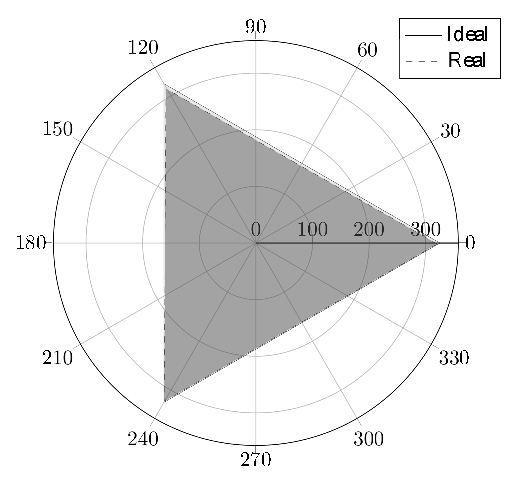
\includegraphics[width=\textwidth]{Unblance_EPS_Pics/EPS_images/square.eps}
                    %\caption{Low correlation with opposed amplitude deviation. The norm values are $G=9322$ and $TDV=0.5198$.}
                    %\label{fig:cases_C}
                %\end{subfigure}
                %~
                %\begin{subfigure}[b]{0.48\textwidth}
                    %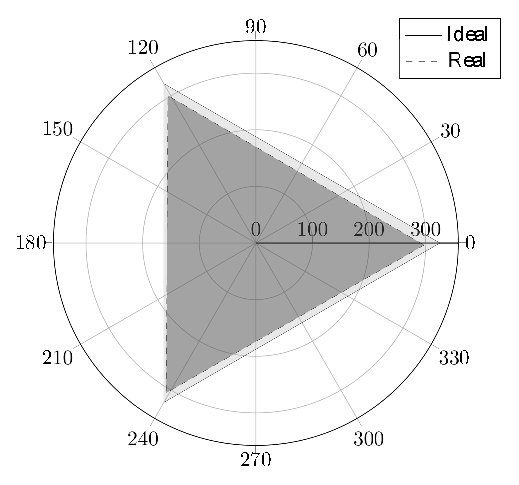
\includegraphics[width=\textwidth]{Unblance_EPS_Pics/EPS_images/circle.eps}
                    %\caption{\centering Low correlation with uniform voltage drop. The norm values are $G=6280$ and $TDV=0.156$.}
                    %\label{fig:cases_D}
                %\end{subfigure}


                \caption{Basic topologies of force commuted rectifiers.}
            \end{figure}

%\begin{figure}[!ht]
        %\centering
        %\includegraphics[width=0.9\textwidth]{EMPC_PNG_Pics/CurrentVoltageRectifiers.png}
        %\caption{Basic topologies of force commuted rectifiers.}
        %\label{BASICCSR:fig:topologies}
    %\end{figure}


As  general case be a front-end  converter power supply (e.g. lighting or telecommunications) shall be designed such that it should have approximately these general characteristics: sinusoidal main currents, unity power factor, high power density and simplicity of the power circuit structure. Two structures are most fitted for the task. First a boost-type input rectifier (e.g., Vienna rectifier, \cite{kolar1996design}), that typically features two $400$ V output voltages with a three-level isolated  DC-DC  converter  or  two  isolated  DC-DC  output  stage (see Fig. \ref{EMPC:fig:network} in Ch.5.). The second candidate is the buck-type  input  rectifier (or current source rectifier (CSR))  (conventionally  six-switch topologies as proposed in \cite{zargari1993current}, \cite{sato1993state}) with only one two-level isolated  DC-DC  converter  output  stage.  Also the  input  stage  can be realized as a three-switch topology with considerably  lower  system  complexity  as  compared  to  the boost-type structure. In particular, the number of utilized active and passive components is much lower. Furthermore, there is no middle-point that has to be stabilized, as this is the case for the boost-type structures, making control and active filter design less complex. Further system advantages are the potential of direct start-up and the implicit over current protection in case of an output short circuit. Therefore, these topologies of high interest for many safety critical applications as such future electric aircraft, or automotive applications or as power supplies for process technology \cite{nussbaumer2007comprehensive}.
The three-switch buck rectifier topology was first proposed in \cite{malesani1987three}. In \cite{itoh1989steady} and \cite{tooth2000effects}, aspects of the system modulation and control have been treated. The application of the topology used as an active filter is discussed in \cite{salo2005three}.  The addition of a DC-DC output boost-stage has been proposed in \cite{baumannnew} in order to maintain 400 V output voltage for a wide input voltage range and for the case of unbalanced mains as, e.g., the loss of one phase.

\myparagraph{Basic operation principles}\label{BASICCSR:sec:OperationPrinciple}

For the derivation of the relative on-times of the three buck transistors $S_i$ with the following assumptions are made for clarity and facilitation of calculations:
\begin{itemize}
	\item The AC-side filter capacitor voltages ($v_{c_p}$, where $p\in\{1,2,3\}$) at the input of the CSR are sinusoidal and in phase with the main harmonic component of voltage.
	
	\begin{equation}
        \begin{array}{rcl}
            v_{c_1}&=&\widehat{v}_c\cos(\omega t)\\
						v_{c_2}&=&\widehat{v}_c\cos(\omega t-2\pi/3)\\
						v_{c_3}&=&\widehat{v}_c\cos(\omega t+2\pi/3),\\
        \end{array}
        \label{BASICMPC:equ:phasorvect}
    \end{equation}
	where $\omega$ is the network voltage's angular velocity.
	
	\item The mains currents are assumed to be equal to the fundamental component of the rectifier input currents.
	\item The current in the DC output inductor $L_{D}$ is not affected by the high frequency ripple due to the switching operation.
\end{itemize}

 For achieving ohmic mains behavior also in case of unbalanced fundamental harmonics conditions the explained modulation method can still be utilized, however, additionally the control structure presented in \cite{baumann2005novel} has to be employed.\\
The waveforms of the phase and line-to-line mains voltages are divided into twelve sectors of $\frac{\pi}{6}$ rad wide shown in Fig.\ref{BASICCSR:fig:waves}. The following calculations are based on the analysis of the first sector which is characterized by the voltage harmonic phase relation. For the remaining sectors the calculations can be accomplished in an similar manner \cite{nussbaumer2007comprehensive}.

\begin{figure}[!ht]
        \centering
        \includegraphics[width=\textwidth]{EMPC_PNG_Pics/Waves.png}
        \caption{Phase voltages $v_{i}$, where line-to-line voltages $v_{N,ij}=v_{N,i}-v_{N,j}$, $(i,j)\in\{R,S,T\}$ and sectors $1$ to $12$ being defined by the different relations of the instantaneous values of the mains phase voltages for $v = 400 V$}
        \label{BASICCSR:fig:waves}
    \end{figure}
		
		Accordingly, on AC side, if conditions are favorable, inductor current can appear in an instant of time either in two out
of three phases or in none. In this modulation technique, the switches in each converter leg can conduct only one at the time (aside from zero states, where both upper and lower switches are conducting). When the upper leg is conducting it is indicated by `$1$', when the lower  `$-1$' and when neither `$0$'. As such the choice whether upper or lower switch of the leg conducts current depends of the reference current vector's sector location.
According to the actual switch combination the DC link current shaped by the choke inductance, and distributed to two of the input phases or the freewheeling diode. With this, the input current space vectors can be calculated for each of the before-mentioned switching states. Generally the space vector of three-phase quantities (e.g., for the rectifier input current) are described as:

\begin{equation}
        \begin{array}{rcl}
            \vec{i}&=&\frac{2}{3}\left(\vec{i}_a+\vec{i}_be^{\frac{j\pi}{3}}+\vec{i}_bc^{\frac{4j\pi}{3}}\right).\\
        \end{array}
        \label{BASICCSR:eqn:currents_all}
    \end{equation}
		
		Based on \ref{BASICCSR:eqn:currents_all} the corresponding active space vectors in the first sector can be obtained as:
		
		\begin{equation}
        \begin{array}{rcl}
            \vec{i}_{(1,0,-1)}=\vec{i}_1&=&2i_{dc}e^{j\pi/6}/\sqrt{3}\\
						\vec{i}_{(0,1,-1)}=\vec{i}_2&=&2i_{dc}e^{j\pi/2}/\sqrt{3}\\
						\vec{i}_{(-1,1,0)}=\vec{i}_3&=&2i_{dc}e^{j5\pi/6}/\sqrt{3}\\
        \end{array}
        \label{BASICCSR:eqn:currents}
    \end{equation}
		
		The resulting discrete space vectors can be used to synthesize desired current
space vector $\vec{i}_{ref}$.

The modulation methods were evaluated in and chosen for this paper based on \cite{moussaoui2005open}, which ensures minimum switching-losses, minimum ripple values of the input capacitor voltages and of the output inductor current. According to this modulation, each pulse interval comprises two active states and a freewheeling state, arranged symmetrically about the middle of the pulse interval (see Table \ref{EMPC:tbl:sequence}). For more in depth functional description see section \ref{EMPC:sec:Modulation}.

\subsection{Coordinate transformations}

In section \ref{EMPC:sec:ModelofCSR} the three phase current source rectifier's (CSR) equations are converted to different coordinate spaces.

\subsubsection{Clarke transformation}\label{BASICCSR:sec:Clarke}

In electrical engineering, Clarke transformation is a mathematical transformation employed to simplify the analysis of three-phase circuits. Conceptually it is similar to the Park transformation. One very useful application is the generation of the reference signal used for space vector modulation control of three-phase inverters. The transformation follows:

\begin{equation}
        \begin{array}{rcl}
            \textbf{i}_{\alpha\beta\gamma}(t)&=&T_{Clarke}\textbf{i}_{abc}(t)
            \begin{bmatrix}
            1& -\frac{1}{2}& -\frac{1}{2}\\
            0& \frac{\sqrt{3}}{2}& -\frac{\sqrt{3}}{2}\\
            \frac{1}{2}& \frac{1}{2}& \frac{1}{2}\\
            \end{bmatrix}
            \begin{bmatrix}
            i_a(t)\\
            i_b(t)\\
            i_c(t)\\
            \end{bmatrix},
        \end{array}
        \label{BASICCSR:eqn:Clarke}
    \end{equation}

    where $\textbf{i}_{abc}$ is the generic three phase current sequence, and $\textbf{i}_{\alpha\beta\gamma}$ is given by the transformation.

    \subsubsection{Park transformation}\label{BASICCSR:sec:Park}

The Park transformation is a tensor that rotates the reference frame of a three-element vector or a three-by-three element matrix in an effort to simplify analysis. The transform can be used to rotate the reference frames of AC waveforms such that they become DC signals. Simplified calculations can then be carried out on these dc quantities before performing the inverse transform to recover the actual three-phase ac results. As an example, the Park transform is often used in order to simplify the analysis of three-phase synchronous machines or to simplify calculations for the control of three-phase inverters. In analysis of three-phase synchronous machines the transformation transfers three-phase stator and rotor quantities into a single rotating reference frame to eliminate the effect of time-varying inductances. The transformation follows:


\begin{equation}
        \begin{array}{rcl}
            \textbf{i}_{dq0}(t)&=&T_{Park}\textbf{i}_{abc}(t)
            \sqrt{\frac{2}{3}}\begin{bmatrix}
            \cos(\theta)& \cos(\theta-\frac{2\pi}{3})& \cos(\theta+\frac{2\pi}{3})\\
            -\sin(\theta)& -\sin(\theta-\frac{2\pi}{3})& -\sin(\theta+\frac{2\pi}{3})\\
            \frac{\sqrt{2}}{2}& \frac{\sqrt{2}}{2}& \frac{\sqrt{2}}{2}\\
            \end{bmatrix}
            \begin{bmatrix}
            i_a(t)\\
            i_b(t)\\
            i_c(t)\\
            \end{bmatrix},
        \end{array}
        \label{BASICCSR:eqn:Park}
    \end{equation}

    where $\theta$ is instantaneous angular position of an arbitrary frequency.

\section{Model based predictive control}

\subsection{Quadratic optimization and predictive control}\label{BASICCSR:sec:MPC}

Philosophically MPC reflects human behavior whereby we select control actions which we think will lead to the best predicted outcome (or output) over some limited horizon. To make this selection we use an internal model of the process in question, and constantly update our decisions as new observations become available. Hence a predictive control law has the following components:
\begin{itemize}
\item The control law depends on predicted behavior.
\item The output predictions are computed using a process model.
\item The current input is determined by optimizing some measure of predicted performance.
\item The receding horizon: the control input is updated at every sampling instant.
\end{itemize}

%\myparagraph{Model predictive control}\label{BASICCSR:sec:MPCOverview}
Most control laws, say PID (proportional, integral and derivative) control, does not explicitly consider the future implication of current control actions. To some extent this is only accounted by the expected closed-loop dynamics. MPC on the other hand
implicitly (or explicitly) computes the predicted behavior over some horizon. One can therefore restrict the choice of the proposed input trajectories to those that do not lead to difficulties in the future.\\
In order to predict the future behavior of a process, we must have a model of how the process behaves. In particular, this model must show the dependence of the output on the current measured variable and the current/future inputs. This does not have to be linear (e.g. transfer function, state-space) and in fact can be just about anything. A precise model is not always required to get tight control, because the decisions are updated regularly. This will deal with some model uncertainty in a fairly fast time scale. The decision on the best control is thus continually updated using information from this comparison \cite{rossiter2017model}.\\
This way, model based predictive control methods are optimal regulators, with a defined cost function on a defined and encompassed prediction horizon with restrictions \cite{kwon2006receding}, \cite{baotic2005optimal}, \cite{herceg2009real}, \cite{grancharova2005survey}. The control signal is calculated over a defined horizon, but from the sequence of applicable control signals only the first one is used in the next sample. This procedure is repeated according to the principle of the moving horizon, using new iterations, as such provides the reaction in each sample. The method was developed for systems with physical restrictions, in the first stage for the control of chemical processes in the oil industry, then it was applied to various rapid processes from automotive or power electronics industry \cite{antoniewicz2009predictive} , \cite{geyer2005low}. By default the optimization problem can be solved, for each sample, or explicitly using the multi-parameter programming techniques (mp-LP, mp-QP).% presented in \textbf{[N-ANNEX 1]-(Needed?)}, over a well-defined parameter space.

	\myparagraph{Linear quadratic optimal control}\label{BASICCSR:sec:LQR}

In practice most MPC algorithms use linear models because the dependence of the predictions on future control choices is then linear and this facilitates optimization as well as off-line analysis of expected closed-loop behavior. However, nonlinear models can be used where the implied computational burden is not a problem and linear approximations are not accurate enough. It is also important to note here the comment fit for purpose. In predictive control, the model is used solely to compute system output predictions, so the model is fit for purpose if it gives accurate enough predictions. The effort and detail put into modeling stage should reflect this.	Let the us assume that the system is linear and time-invariant (LTI):
	
	    \begin{equation}
        \begin{array}{rcl}
            \textbf{x}(q+1)&=&\textbf{Ax}(q)+\textbf{Bu}(q),\\
						%\textbf{y}(q)&=&\textbf{Cx}(q)
        \end{array}
        \label{BASICMPC:equ:basic_LTI}
    \end{equation}

    where $\textbf{x}(q)\in\mathbb{R}^n$ and $\textbf{u}(q)\in\mathbb{R}^m$ are the state and input vectors respectively. We define a quadratic cost function over a finite horizon of $N$ steps:

\begin{equation}
        \begin{array}{rcl}
				%&&\norm{asd}
         J_0(\textbf{U}_0,x(0))&=&\textbf{x}'_N\textbf{P}\textbf{x}_N+\sum^{N-1}_{k=0}\textbf{x}'_k\textbf{Q}\textbf{x}_k+\textbf{u}'_k\textbf{R}\textbf{u}_k\\
        \end{array}
        \label{BASICMPC:equ:cost_function_Euclidian}
    \end{equation}

    where $U_0=[\textbf{u}'_0,\dots,\textbf{u}'_{N-1}]\in\mathbb{R}^s$, $s=m\cdot N$ is the decision vector (with $m$ dimensional input vector) constraining all future inputs, also $\textbf{P}=\textbf{P}'\succeq 0$, $\textbf{Q}=\textbf{Q}'\succeq 0$, $\textbf{R}=\textbf{R}'\succeq 0$, and $\textbf{x}_k$ denotes the state vector at time $k$ obtained form $\textbf{x}_0=\textbf{x}(0)$. We also apply the system model based on \ref{BASICMPC:equ:basic_LTI}:

    \begin{equation}
        \begin{array}{rcl}
            \textbf{x}_{k+1}&=&\textbf{Ax}_k+\textbf{Bu}_k,\\
						%\textbf{y}(q)&=&\textbf{Cx}(q)
        \end{array}
        \label{BASICMPC:equ:basic_horizon model}
    \end{equation}

   From the above a finite optimal control problem can be considered:

   \begin{equation}
        \begin{array}{rcl}
				%&&\norm{asd}
         J^*_0(\textbf{x}(0))&=&\min_{\textbf{U}_0}J_0(\textbf{U}_0,x(0))\\
         &\textnormal{subj. to}&\textbf{x}_{k+1}=\textbf{Ax}_k+\textbf{Bu}_k\\
         &&\textbf{x}_0=\textbf{x}(0)\\
         &&k=0,1,\dots,N-1
        \end{array}
        \label{BASICMPC:equ:optimal_control_problem_Euclidian}
    \end{equation}


    The first step is to write the equality constraints to express all future states and inputs from the initial state $\textbf{x}_0$ until the and of horizon $N$:

    \begin{equation}
        \begin{array}{rcl}
        \underbrace{
        \begin{bmatrix}
        \textbf{x}(0)\\
        \textbf{x}_1\\
        \vdots\\
        \vdots\\
        \textbf{x}_N\\
        \end{bmatrix}}_{\mathcal{X}^x}
        &=&
        \underbrace{
        \begin{bmatrix}
        \textbf{I}_0\\
        \textbf{A}_1\\
        \vdots\\
        \vdots\\
        \textbf{A}^N\\
        \end{bmatrix}}_{\mathcal{S}^x}\textbf{x}(0)+
        \underbrace{
        \begin{bmatrix}
        0& \dots& \dots& 0\\
        \textbf{B}& 0& \dots& 0\\
        \textbf{AB}& \ddots& \ddots& \vdots\\
        \vdots& \ddots& \ddots& \vdots\\
        \textbf{A}^{N-1}\textbf{B}& \ddots& \ddots& \textbf{B}\\
        \end{bmatrix}}_{\mathcal{S}^u}
        \begin{bmatrix}
        \textbf{u}_0\\
        \vdots\\
        \vdots\\
        \textbf{u}_N\\
        \end{bmatrix}.

		\end{array}
        \label{BASICMPC:equ:batch_allstates}
    \end{equation}

    %For the easier notation it is asmued that $\mathcal{X^x}={\textbf{x}(0),\textbf{x}_1,\dots,\textbf{x}_N}$, $\mathcal{S^x}={\textbf{I},\textbf{A},\dots,\textbf{x}_N}$ $ \underbrace{(x + 2)^3}_{\text{text 1}}$
    Here all future states are explicit functions of the state $\textbf{x}(0)$ and the future inputs of $\textbf{u}_0,\textbf{u}_1\cdot$ only. By defining appropriate quantities, we can rewrite \ref{BASICMPC:equ:batch_allstates} in a compact form:

    \begin{equation}
        \begin{array}{rcl}
        \mathcal{X}^x&=&\mathcal{S}^x(0)+\mathcal{S}^u\textbf{U}_0.\\
		\end{array}
        \label{BASICMPC:equ:batch_allstates_compact}
    \end{equation}

    Using the same notation the object function can be rewritten as:

    \begin{equation}
        \begin{array}{rcl}
        J(\textbf{x}_0,\textbf{U}_0)&=&\mathcal{X}'\bar{\textbf{Q}}\mathcal{X}+\textbf{U}_0\bar{\textbf{Q}}\textbf{U}'_0,\\
		\end{array}
        \label{BASICMPC:equ:batch_object}
    \end{equation}

    where $\bar{\textbf{Q}}=diag\{\textbf{Q},\dots,\textbf{Q},\textbf{P}\}$, and $\bar{\textbf{R}}=diag\{\textbf{R},\dots,\textbf{R}\}$. Substituting \ref{BASICMPC:equ:batch_allstates_compact} into the objective function \ref{BASICMPC:equ:batch_object} yields:

    \begin{equation}
        \begin{array}{rcl}
        J(\textbf{x}_0,\textbf{U}_0)&=&(\mathcal{S}^x(0)+\mathcal{S}^u\textbf{U}_0)'\bar{\textbf{Q}}(\mathcal{S}^x(0)+\mathcal{S}^u\textbf{U}_0)+\textbf{U}_0'\bar{\textbf{R}}\textbf{U}_0\\
        &=&\textbf{U}'_0\underbrace{(\mathcal{S}^{u'}\bar{\textbf{Q}}\mathcal{S}^u+\bar{\textbf{R}})}_{\textbf{H}}\textbf{U}_0+ \\
        &+&2\textbf{x}'(0)\underbrace{(\mathcal{S}^{x'}\bar{\textbf{Q}}\mathcal{S}^u)}_{\textbf{F}}\textbf{U}_0+\\
        &+&\textbf{x}'(0)\underbrace{(\mathcal{S}^{x'}\bar{\textbf{Q}}\mathcal{S}^x)}_{\textbf{Y}}\textbf{x}(0)\\
        &=&\textbf{U}'_0\textbf{H}\textbf{U}_0+2\textbf{x}'(0)\textbf{F}\textbf{U}_0+\textbf{x}'(0)\textbf{Y}\textbf{x}(0).
		\end{array}
        \label{BASICMPC:equ:batch_simplfy}
    \end{equation}

    Because $\bar{\textbf{R}}\succ 0$, and $\textbf{H}\succ 0$, thus $J(\textbf{x}_0,\textbf{U}_0)$ is a positive definite quadratic function of $\textbf{U}_0$, therefore its minimum can be found by computing its gradient and setting it to zero, which yields the optimal vector of future inputs:
%
    \begin{equation}
        \begin{array}{rcl}
        \textbf{U}^*_0(\textbf{x}(0))&=&-\textbf{H}^{-1}\textbf{F}'x(0)\\
        &=&-(\mathcal{S}^{u'}\bar{\textbf{Q}}\mathcal{S}^{u}+\bar{\textbf{R}})^{-1}\mathcal{S}^{u'}\bar{\textbf{Q}}\mathcal{S}^{x}\textbf{x}(0).
		\end{array}
        \label{BASICMPC:equ:batch_optimal_solution}
    \end{equation}

    With \ref{BASICMPC:equ:batch_optimal_solution} applied and calculated $\textbf{U}_0$ the cost is the optimal following:

    \begin{equation}
        \begin{array}{rcl}
        \textbf{J}^*_0(\textbf{x}(0))&=&-\textbf{x}(0)'\textbf{F}\textbf{H}^{-1}F'x(0)\\
        &=&\textbf{x}(0)'\left[ \mathcal{S}^{x'}\bar{\textbf{Q}}\mathcal{S}^{x} - \mathcal{S}^{x'}\bar{\textbf{Q}}\mathcal{S}^{u}
        (\mathcal{S}^{u'}\bar{\textbf{Q}}\mathcal{S}^{u}+\bar{\textbf{R}})^{-1}\mathcal{S}^{u'}\bar{\textbf{Q}}\mathcal{S}^{x}  \right]\textbf{x}(0).
		\end{array}
        \label{BASICMPC:equ:batch_optimal_cost}
    \end{equation}

    Note that the optimal vector of future inputs $\textbf{U}^*_0(\textbf{x}(0))$ is a linear function of \ref{BASICMPC:equ:batch_optimal_solution} of the initial state $\textbf{x}(0)$ and the optimal cost $J^*_0(x(0))$ is a quadratic function \ref{BASICMPC:equ:batch_optimal_cost} of the initial state $\textbf{x}(0)$.\\
    Alternatively the formulation can be done in a recursive manner. The optimal cost can be defined as $J^*_j(\textbf{x}_j)$ fot the $j^{th}$ for the $N-j$ step problem starting from state $\textbf{x}_j$ as:

    \begin{equation}
        \begin{array}{rcl}
				%&&\norm{asd}
         J^*_j(\textbf{x}_j)&=&\min_{\textbf{u}_j,\dots,\textbf{u}_{N-1}}\textbf{x}'_N\textbf{P}\textbf{x}_N+\sum^{N-1}_{k=0}\textbf{x}'_k\textbf{Q}\textbf{x}_k+\textbf{u}'_k\textbf{R}\textbf{u}_k.\\
        \end{array}
        \label{BASICMPC:equ:cost_function_Euclidian_recursive}
    \end{equation}

    The optimal "one step cost to go" can be obtained as:

     \begin{equation}
        \begin{array}{rcl}
				%&&\norm{asd}
         J^*_{N-1}(\textbf{x}_{N-1})&=&\min_{\textbf{u}_{N-1}}\textbf{x}'_N\textbf{P}_N\textbf{x}_N+\textbf{x}'_{N-1}\textbf{Q}\textbf{x}_{N-1}+\textbf{u}'_{N-1}\textbf{R}\textbf{u}_{N-1}.\\
          &\textnormal{subj. to}&\textbf{x}_N=\textbf{Ax}_{N-1}+\textbf{Bu}_{N-1}\\
          &&\textbf{P}_N=\textbf{P},\\
        \end{array}
        \label{BASICMPC:equ:cost_function_Euclidian_recursive_onestep}
    \end{equation}

    where $J^*_{N-1}(\textbf{x}_{N-1})$ is a positive quadratic function of the decision variable $\textbf{u}_{N-1}$. Writing \ref{BASICMPC:equ:cost_function_Euclidian_recursive_onestep} as the objective function:

    \begin{equation}
        \begin{array}{rcl}
				%&&\norm{asd}
         J^*_{N-1}(\textbf{x}_{N-1})&=&\min_{\textbf{u}_{N-1}}\{\textbf{x}'_{N-1}(\textbf{A}'\textbf{P}_N\textbf{A}+\textbf{Q})\textbf{x}_{N-1}+\\
         &+&2\textbf{x}'_{N-1}\textbf{A}'\textbf{P}_N\textbf{B}\textbf{u}_{N-1}+\\
         &+&\textbf{u}'_{N-1}(\textbf{B}'\textbf{P}_N\textbf{B}+\textbf{R})\textbf{x}_{N-1}\}.\\
        \end{array}
        \label{BASICMPC:equ:cost_function_Euclidian_recursive_substituted}
    \end{equation}

    The optimal input can be found by setting the gradient to zero:

    \begin{equation}
        \begin{array}{rcl}
        \textbf{u}^*_{N-1}=\underbrace{-(\textbf{B}'\textbf{P}_N\textbf{B}+\textbf{R})^{-1}\textbf{B}'\textbf{P}_N\textbf{A}}_{\textbf{F}_{N-1}}\textbf{x}_{N-1},\\
        \end{array}
        \label{BASICMPC:equ:cost_function_Euclidian_recursive_optimum}
    \end{equation}

    and the optimal one step optimal cost:

    \begin{equation}
        \begin{array}{rcl}
        J^*_{N-1}(\textbf{x}_{N-1})&=&\textbf{x}'_{N-1}\textbf{P}_{N-1}\textbf{x}_{N-1},\\
        \end{array}
        \label{BASICMPC:equ:cost_function_Euclidian_recursive_stepback}
    \end{equation}

    where $\textbf{P}_{N-1}$ can be defined recursively as:

    \begin{equation}
        \begin{array}{rcl}
        \textbf{P}_{N-1}=\textbf{A}'\textbf{P}_N\textbf{A}+\textbf{Q}-\textbf{A}'\textbf{P}_N\textbf{B}(\textbf{B}'\textbf{P}_N\textbf{B}+\textbf{R})^{-1}\textbf{B}'\textbf{P}_N\textbf{A}.\\
        \end{array}
        \label{BASICMPC:equ:cost_function_Euclidian_recursive_P}
    \end{equation}

    The next stage is to write down the "two step" problem based on \ref{BASICMPC:equ:cost_function_Euclidian_recursive_onestep}:

    \begin{equation}
        \begin{array}{rcl}
				%&&\norm{asd}
         J^*_{N-2}(\textbf{x}_{N-2})&=&\min_{\textbf{u}_{N-2}}\textbf{x}'_{N-1}\textbf{P}_{N-1}\textbf{x}_{N-1}+\textbf{x}'_{N-2}\textbf{Q}\textbf{x}_{N-2}+\textbf{u}'_{N-2}\textbf{R}\textbf{u}_{N-2}.\\
          &\textnormal{subj. to}&\textbf{x}_{N-1}=\textbf{Ax}_{N-2}+\textbf{Bu}_{N-2}\\
          %&&\textbf{P}_N=\textbf{P},\\
        \end{array}
        \label{BASICMPC:equ:cost_function_Euclidian_recursive_twostep}
    \end{equation}

    We since \ref{BASICMPC:equ:cost_function_Euclidian_recursive_twostep} has the same form as \ref{BASICMPC:equ:cost_function_Euclidian_recursive_onestep} we can apply the same solution seen at \ref{BASICMPC:equ:cost_function_Euclidian_recursive_optimum}:

    \begin{equation}
        \begin{array}{rcl}
        \textbf{u}^*_{N-2}=\underbrace{-(\textbf{B}'\textbf{P}_{N-1}\textbf{B}+\textbf{R})^{-1}\textbf{B}'\textbf{P}_{N-1}\textbf{A}}_{\textbf{F}_{N-2}}\textbf{x}_{N-2},\\
        \end{array}
        \label{BASICMPC:equ:cost_function_Euclidian_recursive_optimum_twostep}
    \end{equation}

    where the "two step" cost:

    \begin{equation}
        \begin{array}{rcl}
        J^*_{N-2}(\textbf{x}_{N-2})&=&\textbf{x}'_{N-2}\textbf{P}_{N-2}\textbf{x}_{N-2},\\
        \end{array}
        \label{BASICMPC:equ:cost_function_Euclidian_recursive_twostepback}
    \end{equation}

    where $\textbf{P}_{N-2}$ can be defined recursively as:

    \begin{equation}
        \begin{array}{rcl}
        \textbf{P}_{N-2}=\textbf{A}'\textbf{P}_{N-1}\textbf{A}+\textbf{Q}-\textbf{A}'\textbf{P}_{N-1}\textbf{B}(\textbf{B}'\textbf{P}_{N-1}\textbf{B}+\textbf{R})^{-1}\textbf{B}'\textbf{P}_{N-1}\textbf{A}.\\
        \end{array}
        \label{BASICMPC:equ:cost_function_Euclidian_recursive_twoP}
    \end{equation}

    Continuing in this manner at some arbitrary time $k$ the optimal control action is:

    \begin{equation}
        \begin{array}{rcl}
        \textbf{u}^*(k)=\underbrace{-(\textbf{B}'\textbf{P}_{k+1}\textbf{B}+\textbf{R})^{-1}\textbf{B}'\textbf{P}_{k+1}\textbf{A}}_{\textbf{F}_{k}}\textbf{x}_{k},\\
        \end{array}
        \label{BASICMPC:equ:cost_function_Euclidian_recursive_optimum_anystep}
    \end{equation}

    where $k=0,1,\dots,N-1$ and:

    \begin{equation}
        \begin{array}{rcl}
        \textbf{P}_{k}=\textbf{A}'\textbf{P}_{k+1}\textbf{A}+\textbf{Q}-\textbf{A}'\textbf{P}_{k+1}\textbf{B}(\textbf{B}'\textbf{P}_{k+1}\textbf{B}+\textbf{R})^{-1}\textbf{B}'\textbf{P}_{k+1}\textbf{A}.\\
        \end{array}
        \label{BASICMPC:equ:cost_function_Euclidian_recursive_twoP}
    \end{equation}

    and the optimal starting cost starting from the measured state:

     \begin{equation}
        \begin{array}{rcl}
        J^*_{k}(\textbf{x}(k))&=&\textbf{x}'(k)\textbf{P}_{k}\textbf{x}(k).\\
        \end{array}
        \label{BASICMPC:equ:cost_function_Euclidian_recursive_anystepback}
    \end{equation}

    Equation \ref{BASICMPC:equ:cost_function_Euclidian_recursive_twoP} is called the discrete Ricatti equation \cite{borrelli2017predictive}, or Ricatti difference equation, which is initialised with $\textbf{P}_n=\textbf{P}$ and solves backwards. It is worth noting that from \ref{BASICMPC:equ:cost_function_Euclidian_recursive_optimum_anystep} the optimal control action $\textbf{u}^*(k)$ is obtained in the form of feedback law as linear function of the measured state $\textbf{x}(k)$ at time instance $k$, and the optimal cost is \ref{BASICMPC:equ:cost_function_Euclidian_recursive_anystepback}.

	
	\myparagraph{Constrained optimal control}\label{BASICCSR:sec:OptimalControl}
	
	In constrained optimal control for any input action with a given initial state the control action can be computed with quadratic programming but with respect to pre described constraints. As displayed, the linear quadratic approach requires a numerical definition so that a precise calculation can be made, that is, which optimal input trajectory gives the lowest numerical value to the cost. The main requirement is that the cost depends on the batch or recursive input sequence and that low values of cost imply good closed-loop performance good being defined for the process. Of course the choice of the cost affects the complexity of the implied optimization and this is also a consideration.\\
With considering an LTI system such as \ref{BASICMPC:equ:basic_LTI}, let us assume that it is subject to constraints:

\begin{equation}
        \begin{array}{rcl}
            \textbf{x}(q)\in\mathcal{X}^x,&\textnormal{ }\textbf{u}(q)\in\mathcal{U}^u,&\textnormal{ }\forall t\geq0,\\
						%\textbf{y}(q)&=&\textbf{Cx}(q)
        \end{array}
        \label{BASICMPC:equ:basic_LTI_constrained}
    \end{equation}

    where the set of inputs $\mathcal{U}^u\subseteq\mathbb{R}^m$ and states $\mathcal{X}^x\subseteq\mathbb{R}^n$ are polyhedra. when Eucledian norm is used with the cost as \ref{BASICMPC:equ:cost_function_Euclidian} with $\textbf{P}\succeq0$, $\textbf{Q}\succeq0$, and $\textbf{R}\succ0$ we define the constrained optimal control problem as:

    \begin{equation}
        \begin{array}{rcl}
            J^*_0(\textbf{x}(0))&=&\min_{\textbf{U}_0}J_0(\textbf{x}(0),\textbf{U}_0)\\
            &\textnormal{subj. to}&\textbf{x}_{k+1}=\textbf{Ax}_{k}+\textbf{Bu}_{k},k=0,1,\dots,N-1\\
            &&\textbf{x}_N\in\mathcal{X}_f,\textbf{x}_k\in\mathcal{X}^x,\textbf{u}_k\in\mathcal{U}^u\\
            &&\textbf{x}_0=\textbf{x}(0),
        \end{array}
        \label{BASICMPC:equ:constrained_optimal_control_problem}
    \end{equation}

    where $\textbf{x}_N\subseteq\mathbb{R}^n$ is the terminal polyhedral region, and $\textbf{U}_0=[\textbf{u}'_0,\dots,\textbf{u}'_{N-1}]'\in\mathbb{R}^s$ with $s=m\cdot N$ is the optimization vector. We denote $\mathcal{X}_0\subset\mathcal{X}^x$ as the set of initial states $\textbf{x}(0)$ for which the optimal control problem is feasible such as:

    \begin{equation}
        \begin{array}{rcl}
            \mathcal{X}_0&=&\{
            \textbf{x}_0\in\mathbb{R}^n:\exists\textbf{U}_0,\\
            &&s.t.:\textbf{x}_k\in\mathcal{X}^x,\textbf{u}_k\in\mathcal{U}^u,\textbf{x}_N\in\mathcal{X}_f,\\
            &&where\,\textbf{x}_{k+1}=\textbf{Ax}_{k}+\textbf{Bu}_{k},k=0,\dots,N-1
            \}.\\
        \end{array}
        \label{BASICMPC:equ:constrained_initial_set}
    \end{equation}

    We denote $\mathcal{X}_i$ as the set of states $\textbf{x}_i$ at time $i=0,1,\dots,N$ which is feasible for \ref{BASICMPC:equ:constrained_optimal_control_problem}. The sets $\mathcal{X}_i$ are independent of the cost function as long as it guaranties the exsistence of a minima and the algorithm used to compute the solution. There are also ways to define an compute $\mathcal{X}_i$. With the batch approach is as follows:

    \begin{equation}
        \begin{array}{rcl}
            \mathcal{X}_i&=&\{
            \textbf{x}_i\in\mathbb{R}^n:\exists\textbf{U}_i,\\
            &&s.t.:\textbf{x}_k\in\mathcal{X}^x,\textbf{u}_k\in\mathcal{U}^u,\textbf{x}_N\in\mathcal{X}_f,\\
            &&where\,\textbf{x}_{k+1}=\textbf{Ax}_{k}+\textbf{Bu}_{k},k=0,\dots,N-1
            \}.\\
        \end{array}
        \label{BASICMPC:equ:constrained_feasible_set}
    \end{equation}

    This definition requires, that for any initial $\textbf{x}_i\in\mathcal{X}_i$ state there exsists a feasible $\textbf{U}_i=[\textbf{u}_i,\dots,\textbf{u}_{N-1}]$ which keeps the state evolution in the feasible set $\mathcal{X}^x$ at future time instants $k$ and forces $\textbf{x}_N$ into $\mathcal{X}_f$ at $k=N$.\\
    Next we show how to compute $\mathcal{X}_i$ for $i=0,\dots,N-1$. It is stated that the state $\mathcal{X}^x$, $\mathcal{X}_f$ and input $\mathcal{U}^u$ sets are $\mathcal{H}$-polyhedra \cite{borrelli2017predictive}, and $\textbf{A}_x\leq\textbf{x}\textbf{b}_x$, $\textbf{A}_f\textbf{x}_N\leq \textbf{b}_f$, are the set of equality and inequality constraints for the states and the terminal state and $\textbf{A}_u\textbf{u}\leq \textbf{b}_u$ are the set of of equality and inequality constraints on inputs respectively. We define the set of constraints as polyhedron $\mathcal{P}^c_i$ at time instance $i$ as:

    \begin{equation}
        \begin{array}{rcl}
            \mathcal{P}^c_i&=&\{
            (\textbf{U}_i,\textbf{x}_i)\in\mathbb{R}^{m\cdot(N-i)+n},s.t.:\textbf{G}_u\textbf{U}_i-\textbf{E}_i\textbf{x}_i\leq\textbf{w}_i
            \},
        \end{array}
        \label{BASICMPC:equ:constrained_constraint_set}
    \end{equation}

    where $\textbf{G}_i$, $\textbf{E}_i$, and $\textbf{w}_i$ as the matrices of inequality and equality constraints are defined as:

    \begin{equation}
    \begin{small}
        \begin{array}{rcl}
            \textbf{G}_i=\begin{bmatrix}
            \textbf{A}_u& 0& \cdots & 0\\
            0& \textbf{A}_u& \cdots & 0\\
            \vdots& \vdots& \ddots& \vdots\\
            0& 0& \cdots& \textbf{A}_u\\
            0& 0& \cdots& 0\\
            \textbf{A}_x\textbf{B}& 0& \cdots& 0\\
            \textbf{A}_x\textbf{A}\textbf{B}& \textbf{A}_x\textbf{B}& \cdots& 0\\
            \vdots& \vdots& \ddots& \vdots\\
            \textbf{A}_f\textbf{A}^{N-i-1}\textbf{B}& \textbf{A}_f\textbf{A}^{N-i-2}\textbf{B}& \cdots& \textbf{A}_f\textbf{B}\\
            \end{bmatrix}&
            \textbf{E}_i=\begin{bmatrix}
            0\\
            0\\
            \vdots\\
            0\\
            -\textbf{A}_x\\
            -\textbf{A}_x\textbf{A}\\
            -\textbf{A}_x\textbf{A}^2\\
            \vdots\\
            -\textbf{A}_f\textbf{A}^{N-i}\\
            \end{bmatrix}&
            \textbf{w}_i=\begin{bmatrix}
            \textbf{b}_u\\
            \textbf{b}_u\\
            \vdots\\
            \textbf{b}_u\\
            \textbf{b}_x\\
            \textbf{b}_x\\
            \textbf{b}_x\\
            \vdots\\
            \textbf{b}_f\\
            \end{bmatrix}.
        \end{array}
        \label{BASICMPC:equ:constrained_constraint_matrices}
        \end{small}
    \end{equation}

    Also, the set $\mathcal{X}_i$ is a polyhedron serves as the projection of $\mathcal{P}^c_i$ in \ref{BASICMPC:equ:constrained_constraint_set} and in \ref{BASICMPC:equ:constrained_constraint_matrices}.\\
    Next the previously mentioned terms are implemented with using the Euclidian norm case. For this we start with the constrained control problem \ref{BASICMPC:equ:constrained_optimal_control_problem} with the assumption of $\textbf{Q}=\textbf{Q}'\succeq0$, $\textbf{R}=\textbf{R}'\succ0$, and $\textbf{R}=\textbf{R}'\succeq0$. As such the constrained control problem with euclidian norm:

    \begin{equation}
        \begin{array}{rcl}
            J^*_0(\textbf{x}(0))&=&\min_{\textbf{U}_0}J_0(\textbf{x}(0),\textbf{U}_0)=
            \textbf{x}'_N\textbf{P}\textbf{x}_N+\sum^{N-1}_{k=0}\textbf{x}'_k\textbf{Q}\textbf{x}_k+\textbf{u}'_k\textbf{R}\textbf{u}_k\\
            &\textnormal{subj. to}&\textbf{x}_{k+1}=\textbf{Ax}_{k}+\textbf{Bu}_{k},k=0,1,\dots,N-1\\
            &&\textbf{x}_N\in\mathcal{X}_f,\textbf{x}_k\in\mathcal{X}^x,\textbf{u}_k\in\mathcal{U}^u\\
            &&\textbf{x}_0=\textbf{x}(0).
        \end{array}
        \label{BASICMPC:equ:constrained_optimal_control_problem_Euclidian}
    \end{equation}

    As shown in the unconstrained case \ref{BASICMPC:equ:constrained_optimal_control_problem_Euclidian} can be rewritten as:

\begin{equation}
    \begin{array}{rcl}
            %J^*_0(\textbf{x}(0))=
            \min_{\textbf{U}_0}J_0(\textbf{x}(0),\textbf{U}_0)&=& \textbf{U}'_0\textbf{H}\textbf{U}_0+2\textbf{x}(0)\textbf{F}\textbf{U}_0+\textbf{x}(0)\textbf{Y}\textbf{x}(0)\\
            &=&[\textbf{U}'_0\textbf{x}'(0)]
            \begin{bmatrix}
            \textbf{H}&\textbf{F}'\\
            \textbf{F}&\textbf{Y}\\
            \end{bmatrix}
            [\textbf{U}'_0\textbf{x}'(0)]'\\.
            &\textnormal{subj. to}&\textbf{G}_0\textbf{U}_0\leq\textbf{w}_0+\textbf{E}_0\textbf{x}(0),
        \end{array}
        \label{BASICMPC:equ:constrained_optimal_control_problem_Euclidian_second form}
    \end{equation}

    with $\textbf{G}_0$, $\textbf{w}_0$, and $\textbf{E}_0$ are defined in \ref{BASICMPC:equ:constrained_constraint_matrices} and $\textbf{H}$, $\textbf{F}$, and $\textbf{Y}$ are defined in \ref{BASICMPC:equ:batch_simplfy}, additionally as $J_0(\textbf{x}(0),\textbf{U}_0)\geq 0$ it follows that $\begin{bmatrix}
            \textbf{H}&\textbf{F}'\\
            \textbf{F}&\textbf{Y}\\
            \end{bmatrix}\succeq 0$.\\
    To obtain problem \ref{BASICMPC:equ:constrained_optimal_control_problem_Euclidian_second form} elimination of equality constraints can be obtained by successive substitution of $\textbf{x}_{k+1}=\textbf{Ax}_{k}+\textbf{Bu}_{k}$, so only an input sequece as decision variables of $\textbf{U}_0=[\textbf{u}_0,\dots,\textbf{u}_{N-1}]$ and $\textbf{x}(0)$ is left as a parameter vector. In general, it might be more efficient to solve the problem the equality and inequality constraints, so that sparsity can be exploited. To aim this, for this lets define the set of inputs and states as $\tilde{\textbf{z}}=[\textbf{x}'_1,\dots,\textbf{x}'_N,\textbf{u}'_0,\dots,\textbf{u}'_{N-1}]$ and rewrite \ref{BASICMPC:equ:constrained_optimal_control_problem_Euclidian} as:

    \begin{equation}
    \begin{array}{rcl}
            J^*_0(\textbf{x}(0))
            &=&[\textbf{U}'_0\textbf{x}'(0)]
            \begin{bmatrix}
            \textbf{H}&\textbf{F}'\\
            \textbf{F}&\textbf{Y}\\
            \end{bmatrix}
            [\textbf{U}'_0\textbf{x}'(0)]'\\.
            &\textnormal{subj. to}&\textbf{G}_{0,eq}\tilde{\textbf{z}}=\textbf{E}_{0,eq}\textbf{x}(0)\\
            &&\textbf{G}_{0,in}\tilde{\textbf{z}}\leq\textbf{w}_{0,in}+\textbf{E}_{0,in}\textbf{x}(0),
        \end{array}
        \label{BASICMPC:equ:constrained_Euclidian_mergedconstraint}
    \end{equation}

    where $\textbf{G}_{0,eq}$, and $\textbf{E}_{0,eq}$, are the equality constraint matrices, and  $\textbf{G}_{0,in}$, $\textbf{E}_{0,in}$, and $\textbf{w}_{0,in}$ are the inequality constraint matrices respectively:

    \begin{equation}
    \begin{small}
    \begin{array}{c}
            \textbf{G}_{0,eq}=\left[\begin{array}{ccccc|ccccc}
            \textbf{I}&&&&&-\textbf{B}&&&&\\
            -\textbf{A}&\textbf{I}&&&&&-\textbf{B}&&&\\
            &-\textbf{A}&\textbf{I}&&&&&\ddots&&\\
            &&\ddots&\ddots&&&&&\ddots&\\
            &&&-\textbf{A}&\textbf{I}&&&&&-\textbf{B}\\
            \end{array}\right],\textbf{E}_{0,eq}=\left[\begin{array}{c}
            \textbf{A}\\
            0\\
            \vdots\\
            0\\
            \end{array}\right],\\
            \\
             \textbf{G}_{0,in}=\left[\begin{array}{ccccc|ccccc}
            0&&&&&0&&&&\\
            \textbf{A}_x&0&&&&0&&&&\\
            &\textbf{A}_x&&&&&0&&&\\
            &&\ddots&\ddots&&&&\ddots&&\\
            &&&\textbf{A}_x&&&&&0&\\
            &&&&\textbf{A}_f&&&&&0\\
            \hline
            0&&&&&\textbf{A}_u&&&&\\
            &0&&&&&\textbf{A}_u&&&\\
            &&\ddots&&&&&\ddots&&\\
            &&&0&&&&&\textbf{A}_u&\\
            &&&&0&&&&&\textbf{A}_u\\
            \end{array}\right],\textbf{w}_{0,in}=\left[\begin{array}{c}
            \textbf{b}_x\\
            \textbf{b}_x\\
            \vdots\\
            \textbf{b}_x\\
            \textbf{b}_f\\
            \hline
            \textbf{b}_u\\
            \textbf{b}_u\\
            \vdots\\
            \textbf{b}_u\\
            \textbf{b}_u\\
            \end{array}\right],\\
            \textbf{E}_{0,in}=\left[\begin{array}{cccc}
             -\textbf{A}'_x&0&\dots&0\\
             \end{array}\right],

        \end{array}
        \end{small}
        \label{BASICMPC:equ:constrained_Euclidian_matrices}
    \end{equation}

    and the constructed cost matrix $\textbf{H}$ as:

    \begin{equation}
    \begin{small}
    \begin{array}{c}
    \bar{\textbf{H}}=\left[\begin{array}{cccc|ccc}
    \textbf{Q}&&&&&&\\
    &\ddots&&&&&\\
    &&\textbf{Q}&&&&\\
    &&&\textbf{P}&&&\\
    \hline
    &&&&\textbf{R}&&\\
    &&&&&\ddots&\\
    &&&&&&\textbf{R}\\
    \end{array}\right].
    \end{array}
    \end{small}
    \label{BASICMPC:equ:constrained_Euclidian_costmatrix}
    \end{equation}

    In the following the state feedback solution starting from the presumed initial state for one minimizing instance $J^*_0(\textbf{x}(0))$ shall be displayed for the constrained quadratic control problem \ref{BASICMPC:equ:constrained_optimal_control_problem_Euclidian} as \ref{BASICMPC:equ:constrained_Euclidian_mergedconstraint}, with $\textbf{G}_0$, $\textbf{E}_0$ $\textbf{w}_0$ as the constraint describing matrices as defined in \ref{BASICMPC:equ:constrained_constraint_matrices} starting from $\textbf{x}(0)$, and $\textbf{H}$, $\textbf{F}$, and $\textbf{Y}$ as the substitute matrices described in \ref{BASICMPC:equ:batch_simplfy}, to acquire the optimal solution.\\
    We view the initial state $\textbf{x}(0)$ as the vector of parameters as our goal to solve \ref{BASICMPC:equ:constrained_optimal_control_problem_Euclidian} for all values of the set of initial states $\textbf{x}(0)\in\mathcal{X}_0$ and make this dependence explicit, with the computation of $\mathcal{X}_0$ in terms of feasibility, described in  \ref{BASICMPC:equ:constrained_feasible_set}.\\
    For convenience let us define the substitutive term $\textbf{z}$ as:

    \begin{equation}
    \begin{array}{rcl}
            \textbf{z}&=&\textbf{U}_0+\textbf{H}^{-1}\textbf{F}'\textbf{x}(0),
        \end{array}
        \label{BASICMPC:equ:constrained_substitute_z}
    \end{equation}

    where $\textbf{z}\in\mathbb{R}^s$ and with this transform \ref{BASICMPC:equ:constrained_optimal_control_problem_Euclidian} to obtain the equivalent control problem:

    \begin{equation}
    \begin{array}{rcl}
            \hat{J}^*(\textbf{x}(0))&=&J^*_0(\textbf{x}(0))-\textbf{x}(0)'(\textbf{Y}-\textbf{F}\textbf{H}^{-1}\textbf{F}')\textbf{x}(0)\\
            &=&\min_{\textbf{z}}\textbf{z}'\textbf{H}\textbf{z}\\
            &\textnormal{subj. to}&\textbf{G}_0\textbf{U}_0\leq\textbf{w}_0+\textbf{S}_0\textbf{x}(0),
        \end{array}
        \label{BASICMPC:equ:constrained_substitute_J}
    \end{equation}

    where $\textbf{S}_0=\textbf{E}_0+\textbf{G}_0\textbf{H}^{-1}\textbf{F}'$. In this transformed problem the initial parameter vector $\textbf{x}(0)$ appears only on right hand side of constraints. In this case \ref{BASICMPC:equ:constrained_substitute_J} is a multi parametric constrained quadratic optimal program that can be solved explicitly by using geometrical means described first by the authors in \cite{bemporad2002explicit}. This shall be discussed in section \ref{BASICCSR:sec:MPP}.

\subsubsection{Receiding horizon control}\label{BASICCSR:sec:RHC}

    All this said, even if we calculate the best optimal step sequence for solving the constrained control problem, there are still uncertainties for the future. Optimization over a finite horizon has the following disadvantages:
		
		\begin{itemize}
			\item Unforeseen problems may occur after the fixed optimization horizon, which may cancel the sequence of order for the 		calculated finished horizon.
		\item After reaching the time defined by the horizon, the law of command is no longer optimal.
		\item Finite horizon optimization is usually used because of the limited computing power is available, and not for theoretical reasons
		\end{itemize}
		
		To prevent this problem, the notion of optimization is introduced on a moving horizon. In each sample $k$ , an optimization problem is solved over a defined horizon $k,\dots,k+N$ to calculate the appropriate command sequence, and only the first command is applied. This results in a moving optimization horizon, which eliminates the issues listed before displayed on Fig.\ref{BASICCSR:fig:RHC}. \\

\begin{figure}[!ht]
        \centering
        \includegraphics[width=.9\textwidth]{EMPC_PNG_Pics/RHC_gray.jpg}
        \caption{Graphycal display of receiding horison control (RHC) idea \cite{borrelli2017predictive}.}
        \label{BASICCSR:fig:RHC}
    \end{figure}

The Formulation of the optimal control problem with moving horizon \cite{goodwin2006constrained} in the system \ref{BASICMPC:equ:basic_LTI} with input and output constraints as mentioned in \ref{BASICMPC:equ:basic_LTI_constrained} with the cost function to minimize:
		
		\begin{equation}
        \begin{array}{rcl}
				J(\textbf{U},\textbf{x}(q))&=&\min_{\textbf{U}_{q\rightarrow q+N|q}}J_q(\textbf{x}(q),\textbf{U}_{q\rightarrow q+N|q})\\
                &=&\textbf{x}'_{q+N_y|q}\textbf{P}\textbf{x}_{q+N_y|q}+\sum^{N_y-1}_{k=0}\textbf{x}'_{q+k|q}\textbf{Q}\textbf{x}_{q+k|q}+\textbf{u}'_{q+k}\textbf{R}\textbf{u}_{q+k},\\
				&\textnormal{subj. to}&\textbf{x}_N\in\mathcal{X}_f,\textbf{x}_k\in\mathcal{X}^x,\textbf{u}_k\in\mathcal{U}^u\\
				&&\textbf{x}_{q|q}=\textbf{x}(q),\\
				&&\textbf{x}_{q+k+1|q}=\textbf{A}\textbf{x}_{q+k|q}+\textbf{B}\textbf{u}_{q+k},\\
				%&&\textbf{y}_{q+k|q}=\textbf{C}\textbf{x}_{q+k|q}, k\geq0,\\
				&&\textbf{u}_{q+k}=-K\textbf{x}_{q+k|q}, N_u\leq k\leq N_y,\\
        \end{array}
        \label{BASICMPC:equ:receiding_horison_problem}
    \end{equation}
		
		where $\textbf{Q}=\textbf{Q}'\geq0$, $\textbf{R}=\textbf{R}'\geq0$, $\textbf{P}\geq0$, $(\textbf{C},\textbf{A})$ is observable, and $N_u\leq N_y$, $N_c\leq N_y-1$. One trivial possibility to choose $K=0$ and $\textbf{P}$ to satisfy the Lyapunov equation:
		
		\begin{equation}
        \begin{array}{rcl}
				\textbf{P}&=&\textbf{A}'\textbf{PA}+\textbf{Q}\\
        \end{array}
        \label{BASICMPC:equ:receiding_horison_Lyapunov}
    \end{equation}
		
		This means that after $N_u$ samples the control stops and the system is evolving to an open loop form. It is obvious that the choice only makes sense if the open loop system is stable. The second option would as described with the method \ref{BASICMPC:equ:cost_function_Euclidian_recursive_twoP}, but this involves to use an unconstrained control for $N_u$ LQR samples. As a result, the MPC law calculates the optimal command sequence:
		
		\begin{equation}
        \begin{array}{rcl}
				\textbf{U}^*(q)&=&\left\{\textbf{u}^*_q,\dots,\textbf{u}^*_{q+N_u-1}\right\},\\
        \end{array}
        \label{BASICMPC:equ:receiding_optimal_sequence}
    \end{equation}
		
		and only the first control input is applied:
		
		\begin{equation}
        \begin{array}{rcl}
				\textbf{u}(q)=\textbf{u}^*_q.\\
        \end{array}
        \label{BASICMPC:equ:receiding_optimal_first}
    \end{equation}
		
		The optimal control inputs estimated for future samples are not taken into account and the algorithm is
repeated on the basis of new measurements or a new estimation of the states.	

    \subsubsection{Stability of MPC}\label{BASICCSR:sec:MPCStability}

    	The problem of closed system stability with the predictive control has been extensively studied e.g. in \cite{mayne2000constrained}, \cite{grieder2005stabilizing}. In the first generation of model based controllers, stability was achieved more experimentally by choosing parameters based on previous studies and experiences. In 1988 the Lyapunov stability method for discrete systems were introduced \cite{keerthi1988optimal}, and in 1990 for continuous systems \cite{mayne1990receding} also for continuous systems. \\
    While asymptotic convergence $\lim_{k\rightarrow\infty}\textbf{x}_k=0$ is a desirable property, it is generally not sufficient in practice. We would also like a system to stay in a small neighborhood of the origin when it is disturbed by a little. Formally this is expressed as Lyapunov stability.\\
    For the autonomous system:

    \begin{equation}
    \begin{array}{rcl}
            \textbf{x}_{k+1}&=&g(\textbf{x}_k)\\
            %&\textnormal{subj. to}&g(0)=0,
        \end{array}
        \label{BASICMPC:equ:autonom_system}
    \end{equation}

    where $g(0)=0$. The definition of Lyapunov stability is for the equilibrium point $\textbf{x}=0$ of system \ref{BASICMPC:equ:autonom_system} is:
    \begin{itemize}
    \item stable if, for each $\epsilon>0$, there is a $\varphi>0$ such that:
        \begin{equation}
        \begin{array}{c}
                \norm{\textbf{x}_0}<\varphi\textnormal{ s.t.: }\norm{\textbf{x}_k}<\epsilon,\textnormal{ }\forall k\geq0.
            \end{array}
            \label{BASICMPC:equ:lyapunov_1}
        \end{equation}

    \item unstable if not stable

    \item asymptotically stable if in the set $\boldsymbol{\Omega}\subseteq\mathbb{R}^n$ if its stable and:
       \begin{equation}
        \begin{array}{c}
                \lim_{k\rightarrow\infty}\textbf{x}_k=0,\textnormal{ }\forall\textbf{x}_0\in\boldsymbol{\Omega}.
            \end{array}
            \label{BASICMPC:equ:lyapunov_2}
        \end{equation}

    \item globally asymptotically stable if it is asymptotically stable and $\boldsymbol{\Omega}=\mathbb{R}^n$

    \item exponentially stable if it is stable and there exist constants $\chi>0$ and $\psi\in(0,1)$ such that:
    \begin{equation}
        \begin{array}{c}
                \norm{\textbf{x}_0}<\varphi\textnormal{ s.t.: }\norm{\textbf{x}_k}\leq\chi\norm{\textbf{x}_0}\psi^k,\textnormal{ }\forall k\geq0.
            \end{array}
            \label{BASICMPC:equ:lyapunov_3}
        \end{equation}


    \end{itemize}

    Usually to show Lyapunov stability of the origin for a particular system one constructs a so called Lyapunov function, i.e., a function satisfying the conditions of the following theorem:\\
    Consider the equilibrium point $\textbf{x}=0$ of system \ref{BASICMPC:equ:autonom_system}. Let $\boldsymbol{\Omega}\subset\mathbb{R}^n$ be a closed and bounded set containing the origin. Assume there exists a function $V:\mathbb{R}^n\rightarrow\mathbb{R}$ continuous at the origin, finite for every $\textbf{x}\in\boldsymbol{\Omega}$ and such that:

    \begin{subequations}
    \label{BASICMPC:equ:lyapunov_4_1}
        \begin{align}
                V(0)=0 \label{BASICMPC:equ:lyapunov_4_1_a}\\
                V(\textbf{x})>0,\textnormal{ }\forall\textbf{x}\in\boldsymbol{\Omega}\textbackslash\{0\} \label{BASICMPC:equ:lyapunov_4_1_b}\\
                V(\textbf{x}_{k+1})-V(\textbf{x}_{k})\leq-\chi(\textbf{x}_k),\textnormal{ }\forall\textbf{x}\in\boldsymbol{\Omega}\textbackslash\{0\}, \label{BASICMPC:equ:lyapunov_4_1_c}
        \end{align}
    \end{subequations}

     where $\chi:\mathbb{R}^n\rightarrow\mathbb{R}$ is a continuous positive definite function, then $\textbf{x}=0$ is asymptotically stable. As such a function satisfying \ref{BASICMPC:equ:lyapunov_4_1} is called a Lyapunov function.\\
     A similar theorem can be derived for global asymptotic stability i.e.: $\boldsymbol{\Omega}=\mathbb{R}^n$:
     Consider the equilibrium point $\textbf{x}=0$ of system \ref{BASICMPC:equ:autonom_system}. Let $\boldsymbol{\Omega}\subset\mathbb{R}^n$ be a closed and bounded set containing the origin. Assume there exists a function $V:\mathbb{R}^n\rightarrow\mathbb{R}$ continuous at the origin, finite for every $\textbf{x}\in\boldsymbol{\Omega}$ and such that:

     \begin{subequations}
    \label{BASICMPC:equ:lyapunov_4_2}
        \begin{align}
                \norm{\textbf{x}}\rightarrow\infty,\textnormal{ s.t.: }V(\textbf{x})\rightarrow\infty \label{BASICMPC:equ:lyapunov_4_2_a}\\
                V(0)=0 \label{BASICMPC:equ:lyapunov_4_2_b}\\
                V(\textbf{x})>0,\textnormal{ }\forall\textbf{x}\neq0 \label{BASICMPC:equ:lyapunov_4_2_c}\\
                V(\textbf{x}_{k+1})-V(\textbf{x}_{k})\leq-\chi(\textbf{x}_k),\textnormal{ }\forall\textbf{x}\neq0, \label{BASICMPC:equ:lyapunov_4_2_d}
            \end{align}
            \end{subequations}
     where $\chi:\mathbb{R}^n\rightarrow\mathbb{R}$ is a continuous positive definite function, then $\textbf{x}=0$ is globally asymptotically stable.\\
     For linear systems a simple and effective Lyapunov function can be:

     \begin{equation}
        \begin{array}{rcl}
                V(\textbf{x})&=&\textbf{x}'\textbf{P}\textbf{x},\textbf{P}\succ 0,\\
            \end{array}
            \label{BASICMPC:equ:lyapunov_5}
        \end{equation}

    In order to test the satisfaction of the last point of \ref{BASICMPC:equ:lyapunov_4_2}, we compute:

    \begin{equation}
        \begin{array}{rcl}
                V(\textbf{x}_{k+1})-V(\textbf{x}_{k})&=&\textbf{x}'_{k+1}\textbf{P}\textbf{x}_{k+1}-\textbf{x}'_{k}\textbf{P}\textbf{x}_{k}\\
                &=&\textbf{x}'_{k}(\textbf{A}'\textbf{P}\textbf{A})\textbf{x}_{k}-\textbf{x}'_{k}\textbf{P}\textbf{x}_{k}\\
                &=&\textbf{x}'_{k}(\textbf{A}'\textbf{P}\textbf{A}-\textbf{P})\textbf{x}_{k},
            \end{array}
            \label{BASICMPC:equ:lyapunov_6}
        \end{equation}

    therefore, if \ref{BASICMPC:equ:lyapunov_5} holds true then:

    \begin{equation}
        \begin{array}{rcl}
                 \textbf{A}'\textbf{P}\textbf{A}-\textbf{P}&=&-\textbf{Q},\textbf{Q}\succ 0,\\
            \end{array}
            \label{BASICMPC:equ:lyapunov_7}
        \end{equation}

which is referred as discrete time Lyapunov equation. 
\input{subtex/4_b_explicit_CSR_core.tex}
\newpage
\section{Notations used in the chapter}
		
		%\begin{longtable}{r|l}
  % after \\: \hline or \cline{col1-col2} \cline{col3-col4} ...
  %Chapter 4.1. notations&\\
  \begin{scriptsize}
\begin{tabularx}{\textwidth}{r|X}
  
  %%A
  $\textbf{A}$                  & State matrix of the DC side system\\
  $\textbf{A}_d$                & Discretised state matrix of the DC side system\\
  $\textbf{A}_x$              & Constraint state matrix\\
  $\textbf{A}_u$              & Constraint input matrix\\
  $\textbf{A}_f$              & Constraint state matrix at the end of the horizon\\
  $\mathcal{A}$               & Set if indices in states where the constraints are active\\
  $\mathcal{A}^N$               & Set if indices in states where the constraints are inactive\\
  
  %%B
  $\textbf{B}$                  & Input matrix of the DC side system\\
  $\textbf{B_d}$                & Discretised input matrix of the DC side system\\
  
  %%C
  $C_{ac}$                          & AC side inductance\\
  $C_{dc}$                          & DC side inductance\\
  $\textbf{C}$                  & Output matrix of the DC side system\\
  $\textbf{C_d}$                & Discretised output matrix of the DC side system\\
  $C_{reg_i}$                       & Critical region\\
  
  %%D
  $D(-\Theta)$                      & Inverse Clarke transformation\\
  
  %%E
  $\textbf{E}$                & Unified constraint state matrix \\
  
  %%F
  $\textbf{F}$                & State coefficient matrix for calculating the optimal input \\
  $f$                               & Network voltage frequeny\\
  $fpwm$                            & Rectifier switching frequency\\
  $f_s$                             & Simulation frequency\\
  $f_i$                             & Function of state at the $i^th$ step\\
  
  %%G
  $\textbf{G}$                & Unified constraint input matrix \\
  $g_i$                             & Function of input at the $i^th$ step\\
  
  %%H
  $H$                               & Supplementary quadratic optimizer matrix\\
  $HPF(s)$                          & High pass filter transfer function\\
  
  %I
  $i_{abc}$                         & Generic three phase current\\
  $i_{ac_{1,2,3}}$                  & AC side inductance current\\
  $i_{ac_{\alpha,\beta}}$           & AC side inductance current in Clarke frame\\
  $i_{ac_{d,q}}$                    & AC side inductance current in Park frame\\
  $i_{HPF}$                         & AC side damping current\\
  $i_{r_{1,2,3}}$                   & Rectifier current\\
  $i_{rMPC_d}$                      & Direct component of the output of the EMPC controller\\
  $i^*_{r_{1,2,3}}$                 & Rectifier reference current\\
  $i^*_{r_{\alpha,\beta}}$          & Rectifier reference current in Clarke frame\\
  $i_{rcontrol_d}$                  & Direct component of the output of the DC voltage controller\\
  $i_{rHF_d}$                       & Direct component of the damping current of AC noise\\
  $i_{dc}$                          & DC side inductance current\\
  $i_{ref_{\alpha,\beta,\gamma}}$   & $\alpha$, $\beta$, or $\gamma$ component of the reference current vector respecively\\
  $i_{dq0}$                         & Three phase current converted to Park frame\\
  $\vec{i}_{0,\dots,9}$             & Current vector of the phasor\\
  $\vec{i}_{ref}$                   & Reference current vector\\
  
  %%J
  $\mathcal{J}$                     & Set if indices of active constraints\\
  $J$                               & Quadratic EMPC cost function\\
  $J^*$                             & Optimal cost value\\
  $J_0$                             & Cost function to optimize at the initial state\\
  $J^*_0$                           & Optimal cost function at the initial state\\
  
  %%K
  $\mathcal{K}$                     & Set of controller gains respective to critical regions\\
  $K$                               & Feedback gain of EMPC controller\\
  $k_{1,2,3}$                       & State feedback controller's coefficients\\
  
  %L
  $L_{ac}$                          & AC side inductance\\
  $L_{dc}$                          & DC side inductance\\
  $L_S$															& Input filter inductance of the three phase alternating current in VSR\\
  $L_D$															& Inductor for filtering the output current of the CSR (Choke)\\
  
  %%N
  $N$                               & Control horizon\\
  $N_y,N_u,N_c$                     & Output, input and constraint horizons\\
  $n$                               & Current phasor sector indicator\\
  
  %%P
  $\mathcal{P}^c$               & Set of all (input and state) constraints at time instance\\
  $\mathcal{P}_p$             & Set of primary feasibility conditions\\
  $\mathcal{P}_d$             & Set of dual feasibility conditions\\
  $P_n$                             & Nominal power of the CRS\\
  $\textbf{P}$                    & Terminal penalising weight matrix\\
  $\textbf{P}_N$                    & Terminal penalising weight matrix at the end of the horizon\\
  
  %%Q
  $\textbf{Q}$                & State weight matrix of quadratic MPC cost function\\
    $\bar{\textbf{Q}}$                    & Batch of state penalising weight matrix\\
  
  %%R
  $R$                               & Phase resistance\\
  $R_H$                             & Virtual damping resistance\\
  $R_{load}$                        & Load resistance\\
  $\textbf{R}$                & Input weight matrix of quadratic MPC cost function\\
  $\bar{\textbf{R}}$                    & Batch of input penalising weight matrix\\
  $\mathbb{R}$                      & Set of real numbers\\
  
  %%S
  $S$                               & Current phasor sector\\
  $\textbf{S}$                  & Coefficient constraint matrix\\
  $\mathcal{S}^x$             & Set of all possible future state matrices stepping through the horizon\\
  $\mathcal{S}^u$             & Set of all possible future input matrices stepping through the horizon\\
  
  %%T
  $T_s$                             & Switching period\\
  $T_{0,\dots,9}$                   & Dwell time in the corresponding sector\\
  $t$                               & Discrete timestep\\
  
  %%U
  $U$                               & Set of MPC inputs\\
  $Un$                              & Network line-to-line voltage\\
  $\textbf{U}^*_0$            & Optimal vector of future inputs starting from the initial state\\
  $\mathcal{U}^u$             & Set of inputs not violating constraints\\
  $\textbf{u}^*$                & Optimal vector of input\\
  $\widehat{u}$				 & Peak value of AC-side capacitor voltage\\
  $\textbf{u}$                  & Output vector of the DC side system\\
  $u_{1,2,3}$                       & AC side phase voltage\\
  $u_{\alpha,\beta}$                & AC side phase voltage in Clarke frame\\
  $u_{d,q}$                         & AC side phase voltage in Park frame\\
  $u_{c_{1,2,3}}$                   & AC side capacitance voltage\\
  $u_{c_{\alpha,\beta}}$            & AC side capacitance voltage in Clarke frame\\
  $u_{c_{d,q}}$                     & AC side capacitance voltage in Park frame\\
  $u_0$                             & DC side voltage on load\\
  $u^*_0$                           & DC side voltage reference\\
  $u_{MPC}$                         & MPC control variable\\
  $\textbf{u}^*$                & Optimal input vector\\
  
  %%V
  $v_D$								& Output voltage before the choke inductor $L_D$\\
  $v_{i,j}$							& Three phase phase-to-neutral voltage $i,j\in\{R,S,T\}$\\
  $v_{N,RS}$						& Three phase line-to-line voltage of $R$ and $S$\\
  $v_{c_p}$							& AC-side capacitor voltage, where $p\in\{1,2,3\}$\\
  $\hat{v}$							& Voltage peak\\
  
  %%W
  $\textbf{w}$                & Unified constraint vector \\
  
  %%X
  $\mathcal{X}^x$             & Set of all possible future states stepping through the horizon\\
  $\mathcal{X}_f$             & Set of all possible future states at the end of the horizon\\
  $\mathcal{X}_0$             & Set of initial states\\
  $\textbf{x}$											& State vector of a linear time invariant model\\
  $\bar{\textbf{x}}$											& Minimum state value of the objective function\\
  $\textbf{x}(0)$                 & Initial state\\
  
  %%Y
  $\textbf{y}$                  & Input vector of the DC side system\\
  $\textbf{Y}$                  & Remainder supplementary matrix\\
  
  %%Z
  $\textbf{z}$                  & Vector of optimization variables\\
  $\textbf{Z}^*$              & Set of optimizers leading to feasible states\\
  $\textbf{z}$											& Optimizer of linear multi parametric problem\\
  $\tilde{\textbf{z}}$        & Set of all future states and inputs over the horizon\\
  
  %%Greek
  $\delta_{1,2,3}$                  & Conduction state leg\\
  $\delta_{\alpha,\beta}$           & Conduction state leg in Clarke frame\\
  $\delta_{d,q}$                    & Conduction state leg in Park frame\\
  $\theta$                          & Network voltage vector’s angular displacement\\
  $\epsilon,\varphi,\chi,\psi$               & Constant sets\\
  $\Omega$                          & Closed and bounded set of states containing the origin\\
  $\omega$                          & Network voltage vector’s angular velocity\\
  $\omega_{ac}$                     & Ac side LC filter angular velocity\\
  $\omega_{n}$                      & Damping angular velocity\\
  \end{tabularx}
  \end{scriptsize} 

% Summary
\chapter{Summary}
Stuff you need to remember.
 %--> List of thesis and own publications moved here <=====

%% Appendix
\chapter*{Appendix}

\section{Geometric approach to multi parametric programming}\label{BASICCSR:sec:MPP}
    % Section's main text due to more comprehensible source

    In this section the goal is to explain how to solve multi-parametric optimization problems (mp-OP). By start lets consider the following linear multip-parametric problem:

        \begin{equation}
    \begin{array}{rcl}
            J^*(\textbf{x})&=&\min_{\textbf{z}}J(\textbf{x},\textbf{z})=\textbf{c}'\textbf{z}\\
            %&=&\frac{1}{2}\textbf{z}'\textbf{H}\textbf{z}\\
            &\textnormal{subj. to}&\textbf{Gz}\leq\textbf{w}+\textbf{Sx},
        \end{array}
        \label{BASICMPC:equ:MPP_program}
    \end{equation}

    where $\textbf{z}\in\mathbb{R}^s$ is the vector of the optimization variables,  $\textbf{x}\in\mathbb{R}^n$ is the vector of parameters, and of course $J(\textbf{x},\textbf{z}):\mathbb{R}^{s+n}\rightarrow\mathbb{R}$ is the objective or cost function. Additionally $\textbf{G}\in\mathbb{R}^{m\cdot s}$, $\textbf{w}\in\mathbb{R}^m$, $\textbf{c}\in\mathbb{R}^s$ and $\textbf{S}\in\mathbb{R}^{m\cdot n}$ as described in section \ref{BASICCSR:sec:OptimalControl}. Next we define a closed convex parameter set $\textbf{K}\subset\mathbb{R}^n$ such as:

    \begin{equation}
    \begin{array}{rcl}
            \textbf{K}&=&\left\{ \textbf{x}\in\mathbb{R}^n:\textbf{Tx}\leq\textbf{Z}\right\},
        \end{array}
        \label{BASICMPC:equ:MPP_parameterset}
    \end{equation}

    where $\textbf{K}^*\subseteq\textbf{K}$ is the set where \ref{BASICMPC:equ:MPP_program} is feasible, and $\textbf{x}^*\in\textbf{K}^*$ where $\textbf{x}^*$ is the optimum. It is further assumed that:

    \begin{enumerate}
    \item the constraint $\textbf{x}\in\textbf{K}$ is included in the constraints of $\textbf{Gz}\leq\textbf{w}+\textbf{Sx}$.
    \item $\textbf{K}$ is a full dimensional polytope, or the problem can be reformulated to $\textbf{K}$ to be full dimensional with a smaller set of parameters.
    \item $\textbf{S}$ is on full rank, or the problem can be reformulated to $\textbf{S}$ to be full rank with a smaller set of parameters.
    \end{enumerate}

    As such $\textbf{J}^*:\textbf{K}^*\rightarrow\mathbb{R}$ is a function which gives the optimum by $\textbf{x}$. That said let $\textbf{Z}^*:\textbf{K}^*\rightarrow\mathbb{R}^s$ the function which gives the set of optimizers namely $\textbf{z}^*\in\textbf{Z}^*$. The task is to find a $\textbf{K}^*\subseteq\textbf{K}$ set and a $\textbf{z}^*\in\textbf{Z}^*$ optimizer and the value of the optimum.\\
    Beside of the systematic linear and quadratic program solutions \cite{borrelli2017predictive} there is a direct geometrical solution for the problem which uses critical regions for describing the parameter space. The critical regions are convex subsets of the parameter space where the optimum is constant based on the function of the parameters.
    Consider the multi parametric program \ref{BASICMPC:equ:MPP_program}, and let $\mathcal{I}_c=\{1,\dots,m\}$ be the set of constraint indices. For any $\mathcal{A}\subseteq\mathcal{I}_c$, let $\textbf{G}_{\mathcal{A}}$, and $\textbf{S}_{\mathcal{A}}$ be the subsets of $\textbf{G}$, and $\textbf{S}$, respectively, compromising the rows indexed by $\mathcal{A}$, and denote with $\textbf{G}_j$, $\textbf{S}_j$ and $\textbf{w}_j$, the $j^{th}$ row of $\textbf{G}$, $\textbf{S}$ and $\textbf{w}$. We define $\mathcal{C}_{\mathcal{A}}$ as the set of states $\textbf{x}$ for which the same set $\mathcal{A}$ of constraints is active at the optimum. Formally, the \emph{optimal partition} of $\mathcal{I}_c$ at $\textbf{x}$ is the optimal partition of $(\mathcal{A}(x),\mathcal{A}^N(x))$, where:

    \begin{equation}
    \begin{array}{rcl}
            \mathcal{A}&=&\{j\in\mathcal{I}_c:\textbf{G}_j\textbf{z}^*(x)-\textbf{S}_j\textbf{x}=\textbf{w}_j\forall\textbf{z}^*\in\textbf{Z}^*(x)\}\\
            \mathcal{A}^N&=&\{j\in\mathcal{I}_c:\exists\textbf{z}^*\in\textbf{Z}^*(x)\textnormal{ s.t.: }\textbf{G}_j\textbf{z}^*(x)-\textbf{S}_j\textbf{x}<\textbf{w}_j\}.
        \end{array}
        \label{BASICMPC:equ:MPP_stateset_optimal partition}
    \end{equation}

    It can be noticed, that $\mathcal{A}$ and $\mathcal{A}^N$ are disjoint (the intersection of $\mathcal{A}$ and $\mathcal{A}^N$ is an empty set) and they union is $\mathcal{I}_c$. As such consider a set $\mathcal{A}\subseteq\mathcal{I}_c$, then the \emph{critical region} associated with the set of active constraints $\mathcal{A}$ is defined as:

    \begin{equation}
    \begin{array}{rcl}
            \mathcal{C}_{\mathcal{A}}&=&\{\textbf{x}\in\textbf{K}^*:\mathcal{A}(x)=\mathcal{A}\}.
        \end{array}
        \label{BASICMPC:equ:MPP_stateset_optimal critical}
    \end{equation}

    With the above the critical region $\mathcal{C}_{\mathcal{A}}$ is the set of all $\textbf{x}$ states such that constraints indexed by $\mathcal{A}$ are active at the optimum of problem \ref{BASICMPC:equ:MPP_program}. Furthermore it can be proven, that the optimum is an affine function in the domain of $\textbf{K}$ adn unique for every critical region. As such the problem can be separated into two parts:

    \begin{enumerate}
    \item Find the least dimension subset of $\textbf{K}$ which contains $\textbf{K}^*$.
    \item Partition $\textbf{K}^*$ into critical regions and find the optimum for every critical region.
    \end{enumerate}

    The graphical representation of critical regions can be observed at Fig.\ref{BASICCSR:fig:Crit}. The algorithm starts from a starting point $\textbf{x}_0$ and solves the linear programming problem and find $\textbf{z}^*(\textbf{x}_0)$. After this find the active constrains and define the corresponding critical region $\mathcal{C}_{\mathcal{A}}(\textbf{x}_0)$. Its clear from the definition of one critical region that $J^*$ is constant for any $\textbf{x}\in\mathcal{C}_{\mathcal{A}}(\textbf{x}_0)$. Next  we find the optimum and the optimizer's value for $\textbf{x}\in\mathcal{C}_{\mathcal{A}}(\textbf{x}_0)$. and move on to the next critical region. If the optimum problem is not degenerate then finding the critical regions is straightforward, but in the contrary the outcome is defined by the algorithm's starting direction.

    \begin{figure}[!ht]
        \centering
        \includegraphics[width=.9\textwidth]{EMPC_PNG_Pics/criticalregions.jpg}
        \caption{Partitioning incrementally the two dimensional parameter space to critical regions from $C0$ to $C11$.}
        \label{BASICCSR:fig:Crit}
    \end{figure}

    As it shall be described in section \oldref{EMPC:sec:main}, the if the linear optimization could be described with quadratic programming the process yield more computational cost efficient results in a lot of cases. As such it is advised to apply above geometrical approach in a multi-parametric quadratic programming (mp-QP) environment, as it would be used in the explicit MPC. Consider a multi parametric quadratic program:

    \begin{equation}
    \begin{array}{rcl}
            J^*(\textbf{x})&=&\min_{\textbf{z}}J(\textbf{x},\textbf{z})=\frac{1}{2}\textbf{z}'\textbf{H}\textbf{z}\\
            &\textnormal{subj. to}&\textbf{Gz}\leq\textbf{w}+\textbf{Sx},
        \end{array}
        \label{BASICMPC:equ:MPQP}
    \end{equation}

    and the variables are defined as by \ref{BASICMPC:equ:MPP_program} additionally it is assumed that $\textbf{H}\succ 0$. The goal is to find the value function $J^*(\textbf{x})$ and the optimizer function $\textbf{z}^*(\textbf{x})$ in $\textbf{K}^*$. The search of these functions proceeds by partitioning the set of feasible states into critical regions as before. Note that the more general problem with $J(\textbf{x},\textbf{z})=\frac{1}{2}\textbf{z}'\textbf{H}\textbf{z}+\textbf{x}'\textbf{F}\textbf{x}$ can always be transformed into \ref{BASICMPC:equ:MPQP} using the variable substitution $\tilde{\textbf{z}}=\textbf{z}+\textbf{H}^{-1}\textbf{F}'\textbf{x}$.\\
    As previously let be $j$ the $j^{th}$ row of a matrix or the $j^{th}$ element in a vector, also $\mathcal{J}=\{1,\dots,m\}$ be the set of constraint indices and for any $\mathcal{A}\subseteq\mathcal{I}_c$, also $\textbf{G}_{\mathcal{A}}$, $\textbf{w}_{\mathcal{A}}$, and $\textbf{S}_{\mathcal{A}}$ be the submatrices of $\textbf{G}$, $\textbf{w}$ and $\textbf{S}$ respectively, consisting rows, indexed by $\mathcal{A}$, and $\textbf{K}^*$ is full dimensional.
    with the definition displayed in \ref{BASICMPC:equ:MPP_stateset_optimal partition}, and \ref{BASICMPC:equ:MPP_stateset_optimal critical} it can be showed that the critical regions of a multi parametric quadratic program are polyhedra. Let $(\mathcal{A},\mathcal{A}^N)=(\mathcal{A}(\bar{\textbf{x}}),\mathcal{A}^N(\bar{\textbf{x}}))$ for some $\bar{\textbf{x}}\in\textbf{K}^*$, where for any given $\bar{\textbf{x}}\in\textbf{K}^*$, $J^*(\bar{\textbf{x}})$ denotes the minimum value of the objective function for $\textbf{x}=\bar{\textbf{x}}$. Then:

    \begin{enumerate}
    \item the closure of $\mathcal{C}_{\mathcal{A}}$ is a polyhedron.
    \item $\textbf{z}^*(\textbf{x})$ is an affine function of the state inside $\mathcal{C}_{\mathcal{A}}$, i.e.: $\textbf{z}^*(\textbf{x})=\textbf{F}_i\textbf{x}+\textbf{g}_i$ for all $\mathcal{C}_{\mathcal{A}}$.
    \item $J^*(\textbf{x})$ is a quadratic function of the state inside $\mathcal{C}_{\mathcal{A}}$, i.e.: $J^*(\textbf{x})=\textbf{x}'\textbf{M}_i\textbf{x}+\textbf{c}_i\textbf{x}+\textbf{d}_i$ for all $\textbf{x}\in\mathcal{C}_{\mathcal{A}}$.
    \end{enumerate}

    For proving the above, the first order Karush-Kuhn-Tucker (KKT) conditions (described in \cite{borrelli2017predictive} in detail) for multi parameter quadratic programs are:

    \begin{subequations}
    \label{BASICMPC:equ:MPP_KKT}
        \begin{align}
        \textbf{Hz}^*+\textbf{G}'\textbf{u}^*=0,\,\textbf{u}\in\mathbb{R}^m        \label{BASICMPC:equ:MPP_KKT_a} \\
        \textbf{u}^*_i(\textbf{G}_i\textbf{z}^*-\textbf{w}_i-\textbf{S}_i\textbf{x})=0,\,i=1,\dots,m \label{BASICMPC:equ:MPP_KKT_b} \\
        \textbf{u}^*\geq 0 \label{BASICMPC:equ:MPP_KKT_c} \\
        \textbf{G}\textbf{z}^*-\textbf{w}-\textbf{S}\textbf{x}\leq 0 \label{BASICMPC:equ:MPP_KKT_d}.
    \end{align}
    \end{subequations}

    With the KKT conditions \ref{BASICMPC:equ:MPP_KKT} the constraints of quadratic problem \ref{BASICMPC:equ:MPQP} can be written as:

    \begin{equation}
        \label{BASICMPC:equ:MPP_KKT_result}
        \begin{aligned}[c]
            \frac{dL}{d\textbf{z}}\geq& 0\\
            \frac{dL}{d\lambda}\geq& 0\\
            \textbf{z}\frac{dL}{d\textbf{z}}=&0\\
            \lambda g_l(\textbf{x})=&0\\
            \textbf{z}\geq0\,,\lambda\geq0&
        \end{aligned}
        \qquad\Longleftrightarrow\qquad
        \begin{aligned}[c]
            \textbf{z}'\textbf{H}+\lambda\textbf{G}\geq&0\\
            \textbf{Gz}-\textbf{w}-\textbf{Sx}\leq&0\\
            \textbf{z}'(\textbf{Hz}+\textbf{G}'\lambda)=&0\\
            \textbf{z}\geq0\,,\lambda\geq0&,
        \end{aligned}
    \end{equation}

    where $\lambda$ is the Lagrange multiplier, $L$ is the Lagrange function and $g(\textbf{x})$ is the equality constraint. Then \label{BASICMPC:equ:MPP_KKT_result} can be applied to the active constraints of \ref{BASICMPC:equ:MPQP} applied on the critical region of $\mathcal{C}_{\mathcal{A}}$:

    \begin{equation}
    \begin{array}{rcl}
            \textbf{Hz}+\textbf{G}'_{\mathcal{A}}\lambda_{\mathcal{A}}&=&0\\
            \lambda_{\mathcal{A}}(\textbf{G}_{\mathcal{A}}\textbf{z}-\textbf{w}_{\mathcal{A}}-\textbf{S}_{\mathcal{A}}\textbf{x})&=&0\\
            \textbf{G}\textbf{z}-\textbf{w}-\textbf{S}\textbf{x}&\leq&0\\
            \lambda_{\mathcal{A}}&\geq&0.
        \end{array}
        \label{BASICMPC:equ:KKT_active}
    \end{equation}

    From \ref{BASICMPC:equ:KKT_active} it follows:

    \begin{equation}
    \begin{array}{rcl}
            \textbf{z}&=&-\textbf{H}^{-1}\textbf{G}'_{\mathcal{A}}\lambda_{\mathcal{A}}\\
            0&=&\lambda_{\mathcal{A}}(-\textbf{G}_{\mathcal{A}}\textbf{H}^{-1}\textbf{G}'_{\mathcal{A}}-\textbf{w}_{\mathcal{A}}-\textbf{S}_{\mathcal{A}}\textbf{x}),
        \end{array}
        \label{BASICMPC:equ:MPP_KKT_result_2}
    \end{equation}

    which then implies that:

    \begin{equation}
    \begin{array}{rcl}
            \lambda_{\mathcal{A}}&=&(-\textbf{G}_{\mathcal{A}}\textbf{H}^{-1}\textbf{G}'_{\mathcal{A}})^{-1}(\textbf{w}_{\mathcal{A}}+\textbf{S}_{\mathcal{A}}\textbf{x})\\
            \textbf{z}&=&-\textbf{H}^{-1}\textbf{G}'_{\mathcal{A}}(-\textbf{G}_{\mathcal{A}}\textbf{H}^{-1}\textbf{G}'_{\mathcal{A}})(\textbf{w}_{\mathcal{A}}+\textbf{S}_{\mathcal{A}}\textbf{x}).
        \end{array}
        \label{BASICMPC:equ:MPP_KKT_result_3}
    \end{equation}

    In this case $\textbf{z}$ serves as the optimum if the KKT conditions are fulfilled. Substituting \label{BASICMPC:equ:KKT_active} into \label{BASICMPC:equ:MPP_KKT_result_3} yields:

    \begin{equation}
    \begin{array}{rcl}
            (-\textbf{G}_{\mathcal{A}}\textbf{H}^{-1}\textbf{G}'_{\mathcal{A}})^{-1}(\textbf{w}_{\mathcal{A}}+\textbf{S}_{\mathcal{A}}\textbf{x})
            &\geq&0\\
            (\textbf{G}_{\mathcal{A}}-\textbf{H}^{-1}\textbf{G}'_{\mathcal{A}})(-\textbf{G}_{\mathcal{A}}\textbf{H}^{-1}\textbf{G}'_{\mathcal{A}})^{-1}(\textbf{w}_{\mathcal{A}}+\textbf{S}_{\mathcal{A}}\textbf{x})
            &\leq&\textbf{w}+\textbf{Sx}.
            \end{array}
        \label{BASICMPC:equ:MPP_KKT_result_4}
    \end{equation}

    This inequality of \ref{BASICMPC:equ:MPP_KKT_result_4} expresses the critical region of $\mathcal{C}_{\mathcal{A}}$, and for said region the optimizer can be expressed as:

    \begin{equation}
    \begin{array}{rcl}
            \textbf{z}^*&=&(-\textbf{H}^{-1}\textbf{G}'_{\mathcal{A}})(-\textbf{G}_{\mathcal{A}}\textbf{H}^{-1}\textbf{G}'_{\mathcal{A}})^{-1}(\textbf{w}_{\mathcal{A}}+\textbf{S}_{\mathcal{A}}\textbf{x}).
            \end{array}
        \label{BASICMPC:equ:MPQP_optimizer}
    \end{equation}

    With this in hand the quiadratic multi parametric program \ref{BASICMPC:equ:MPQP} can be solved the same way as the linear multi parametric program \ref{BASICMPC:equ:MPP_program}, an the optimum value can be calulated for every critical region explicitly, as the affine function of parameters.

%
%    The main idea of multi parametric algorithms is to construct a so called critical region in a neighborhood for a given parameter using necessary and sufficient conditions for optimality, and then recursively explore the parameter space outside of said region, in a geometric fashion.
%
%    \myparagraph{Linearly constrained multi parametric programs}\label{BASICCSR:sec:MPP_Linear}
%
%    Consider a multi parametric optimization program:
%
%    \begin{equation}
%    \begin{array}{rcl}
%            J^*(\textbf{x})&=&\min_{\textbf{z}}J(\textbf{x},\textbf{z})\\
%            %&=&\frac{1}{2}\textbf{z}'\textbf{H}\textbf{z}\\
%            &\textnormal{subj. to}&\textbf{Gz}\leq\textbf{w}+\textbf{Sx},
%        \end{array}
%        \label{BASICMPC:equ:MPP_program}
%    \end{equation}
%
%    where $\textbf{z}\in\mathbb{R}^s$ are the optimization variables,  $\textbf{x}\in\mathbb{R}^n$ is the vector of states, and of course $J(\textbf{x},\textbf{z}):\mathbb{R}^{s+n}\rightarrow\mathbb{R}$ is the objective or cost function. Additionally $\textbf{G}\in\mathbb{R}^{m\cdot s}$, $\textbf{w}\in\mathbb{R}^m$, and $\textbf{S}\in\mathbb{R}^{m\cdot n}$ as described in the previous section. Lets state that the states are in a closed, bounded (constrained), and polyhedral set $\mathcal{K}\subset\mathbb{R}^n$:
%
%    \begin{equation}
%    \begin{array}{rcl}
%            \mathcal{K}&=&\{\textbf{x}\in\mathbb{R}:\textbf{A}_x\leq\textbf{xb}_x\}
%        \end{array}
%        \label{BASICMPC:equ:MPP_stateset}
%    \end{equation}
%
%    and lets $\mathcal{K}^*\subseteq\mathcal{K}$ be the set of parameters such that \ref{BASICMPC:equ:MPP_program} is feasible:
%
%    \begin{equation}
%    \begin{array}{rcl}
%            \mathcal{K}^*&=&\{\textbf{x}\in\mathcal{K}:\exists\textbf{x}\,s.t.:\,\textbf{Gz}\leq\textbf{w}+\textbf{Sx}\}.
%        \end{array}
%        \label{BASICMPC:equ:MPP_stateset_params}
%    \end{equation}
%
%    It is further assumed that:
%    \begin{enumerate}
%    \item the constraint $\textbf{x}\in\mathcal{K}$ is included in the constraints of $\textbf{Gz}\leq\textbf{w}+\textbf{Sx}$.
%    \item $\mathcal{K}$ is a full dimensional polytope, or the problem can be reformulated to $\mathcal{K}$ to be full dimensional with a smaller set of parameters.
%    \item $\textbf{S}$ is on full rank, or the problem can be reformulated to $\textbf{S}$ to be full rank with a smaller set of parameters.
%    \end{enumerate}
%
%    With the above assumptions in mind the following theorem can be stated, where we consider the problem \ref{BASICMPC:equ:MPP_program}, and the domain of $J(\textbf{z},\textbf{x})$ is $\mathbb{R}^{s+n}$, then $\mathcal{K}^*$ is a polyscope. This is because $\mathcal{K}^*$ is the projection of the set $\textbf{Gz}-\textbf{Sx}\leq\textbf{w}$ on the $\textbf{x}$ space intersected with the polytope $\mathcal{K}$. The aim is to determine a feasible set of $\mathcal{K}^*\subseteq\mathcal{K}$ of the states, the expression of the value function $J^*(\textbf{x})$, and the expression of optimizers $\textbf{z}^*\in\textbf{Z}^*$, where $\textbf{Z}^*:\mathcal{K}^*\rightarrow 2^{\mathbb{R}^s}$, yielding $J^*(\textbf{x})$.
%
%    \myparagraph{Definition of critical region}\label{BASICCSR:sec:MPP_Critical}
%
%    Consider the multi parametric program \ref{MPP_program}, and let $\mathcal{I}_c=\{1,\dots,m\}$ be the set of constraint indices. For any $\mathcal{A}\subseteq\mathcal{I}_c$, let $\textbf{G}_{\mathcal{A}}$, and $\textbf{S}_{\mathcal{A}}$ be the submatrices of $\textbf{G}$, and $\textbf{S}$, respectively, compromising the rows indexed by $\mathcal{A}$, and denote with $\textbf{G}_j$, $\textbf{S}_j$ and $\textbf{w}_j$, the $j^th$ row of $\textbf{G}$, $\textbf{S}$ and $\textbf{w}$. We define $\mathcal{C}_{\mathcal{A}}$ as the set of states $\textbf{x}$ for which the same set $\mathcal{A}$ of constraints is active at the optimum. Formally, the \emph{optimal partition} of $\mathcal{I}_c$ at $\textbf{x}$ is the optimal partition of $(\mathcal{A}(x),\mathcal{A}^N(x))$, where:
%
%    \begin{equation}
%    \begin{array}{rcl}
%            \mathcal{A}&=&\{j\in\mathcal{I}_c:\textbf{G}_j\textbf{z}^*(x)-\textbf{S}_j\textbf{x}=\textbf{w}_j\forall\textbf{z}^*\in\textbf{Z}^*(x)\}\\
%            \mathcal{A}^N&=&\{j\in\mathcal{I}_c:\exists\textbf{z}^*\in\textbf{Z}^*(x)\textnormal{ s.t.: }\textbf{G}_j\textbf{z}^*(x)-\textbf{S}_j\textbf{x}<\textbf{w}_j\}.
%        \end{array}
%        \label{BASICMPC:equ:MPP_stateset_optimal partition}
%    \end{equation}
%
%    It can be noticed, that $\mathcal{A}$ and $\mathcal{A}^N$ are disjoint and they union is $\mathcal{I}_c$. As such consider a set $\mathcal{A}\subseteq\mathcal{I}_c$, then the \emph{critical region} associated with the set of active constraints $\mathcal{A}$ is defined as:
%
%    \begin{equation}
%    \begin{array}{rcl}
%            \mathcal{C}_{\mathcal{A}}&=&\{\textbf{x}\in\mathcal{K}^*:\mathcal{A}(x)=\mathcal{A}\}.
%        \end{array}
%        \label{BASICMPC:equ:MPP_stateset_optimal critical}
%    \end{equation}
%
%    With the above the set $\mathcal{C}_{\mathcal{A}}$ is the set of all $\textbf{x}$ states such that constraints indexed by $\mathcal{A}$ are active at the optimum of problem \ref{MPP_program}.
%
%    \myparagraph{Multi parametric quadratic programming}\label{BASICCSR:sec:MPP_QP}
%
%    Lets assume that the objective function is a quadratic function:
%
%    \begin{equation}
%    \begin{array}{rcl}
%            J^*(\textbf{x})&=&\min_{\textbf{z}}J(\textbf{z},\textbf{x})=\\
%            &=&\frac{1}{2}\textbf{z}'\textbf{H}\textbf{z}\\
%            &\textnormal{subj. to}&\textbf{Gz}\leq\textbf{w}+\textbf{Sx},
%        \end{array}
%        \label{BASICMPC:equ:MPP_quadratic}
%    \end{equation}
%
%    and the variables are defined as by \ref{MPP_program} additionally it is assumed that $\textbf{H}\succ 0$. The goal is to find the value function $J^*(\textbf{x})$ and the optimizer function $\textbf{z}^*(\textbf{x})$ in $\mathcal{K}^*$. The search of these functions proceeds by partitioning the set of feasible states into critical regions. Note that the more general problem with $J(\textbf{x},\textbf{z})=\frac{1}{2}\textbf{z}'\textbf{H}\textbf{z}+\textbf{x}'\textbf{F}\textbf{x}$ can always be transformed into \ref{BASICMPC:equ:MPP_quadratic} using the variable substitution $\tilde{\textbf{z}}=\textbf{z}+\textbf{H}^{-1}\textbf{F}'\textbf{x}$.\\
%    As previously let be $j$ the $j^{th}$ row of a matrix or the $j^{th}$ element in a vector, also $\mathcal{J}=\{1,\dots,m\}$ be the set of constraint indices and for any $\mathcal{A}\subseteq\mathcal{I}_c$, also $\textbf{G}_{\mathcal{A}}$, $\textbf{w}_{\mathcal{A}}$, and $\textbf{S}_{\mathcal{A}}$ be the submatrices of $\textbf{G}$, $\textbf{w}$ and $\textbf{S}$ respectively, consisting rows, indexed by $\mathcal{A}$, and $\mathcal{K}^*$ is full dimensional.
%    with the definition displayed in \ref{BASICMPC:equ:MPP_stateset_optimal partition}, and \ref{BASICMPC:equ:MPP_stateset_optimal critical} it can be showed that the critical regions of a multi parametric quadratic program are polyhedra. Let $(\mathcal{A},\mathcal{A}^N)=(\mathcal{A}(\bar{\textbf{x}}),\mathcal{A}^N(\bar{\textbf{x}}))$ for some $\bar{\textbf{x}}\in\mathcal{K}^*$, where for any given $\bar{\textbf{x}}\in\mathcal{K}^*$, $J^*(\bar{\textbf{x}})$ denotes the minimum value of the objective function for $\textbf{x}=\bar{\textbf{x}}$. Then
%    \begin{enumerate}
%    \item the closure of $\mathcal{C}_{\mathcal{A}}$ is a polyhedron.
%    \item $\textbf{z}^*(\textbf{x})$ is an affine function of the state inside $\mathcal{C}_{\mathcal{A}}$, i.e.: $\textbf{z}^*(\textbf{x})=\textbf{F}_i\textbf{x}+\textbf{g}_i$ for all $\mathcal{C}_{\mathcal{A}}$.
%    \item $J^*(\textbf{x})$ is a quadratic function of the state inside $\mathcal{C}_{\mathcal{A}}$, i.e.: $J^*(\textbf{x})=\textbf{x}'\textbf{M}_i\textbf{x}+\textbf{c}_i\textbf{x}+\textbf{d}_i$ for all $\textbf{x}\in\mathcal{C}_{\mathcal{A}}$.
%    \end{enumerate}
%
%    For proving the above, the first order Karush-Kuhn-Tucker (KKT) conditions for multi parameter quadratic programs are:
%
%    \begin{subequations}
%    \label{BASICMPC:equ:MPP_KKT}
%        \begin{align}
%        \textbf{Hz}^*+\textbf{G}'\textbf{u}^*=0,\,\textbf{u}\in\mathbb{R}^m        \label{BASICMPC:equ:MPP_KKT_a} \\
%        \textbf{u}^*_i(\textbf{G}_i\textbf{z}^*-\textbf{w}_i-\textbf{S}_i\textbf{x})=0,\,i=1,\dots,m \label{BASICMPC:equ:MPP_KKT_b} \\
%        \textbf{u}^*\geq 0 \label{BASICMPC:equ:MPP_KKT_c} \\
%        \textbf{G}\textbf{z}^*-\textbf{w}-\textbf{S}\textbf{x}\leq 0 \label{BASICMPC:equ:MPP_KKT_d}.
%    \end{align}
%    \end{subequations}
%
%    Let us assume we have determined the optimal partition, namely $(\mathcal{A},\mathcal{A}^N)=(\mathcal{A}(\bar{\textbf{x}}),\mathcal{A}^N(\bar{\textbf{x}}))$ for some $\bar{\textbf{x}}\in\mathcal{K}^*$. The primary feasibility condition \ref{BASICMPC:equ:MPP_KKT_d} can be rewritten as:
%
%    \begin{subequations}
%    \label{BASICMPC:equ:MPP_KKT_rewritten}
%        \begin{align}
%         \textbf{G}_{\mathcal{A}}\textbf{z}^*-\textbf{S}_{\mathcal{A}}\textbf{x}=\textbf{w}_{\mathcal{A}} \label{BASICMPC:equ:MPP_KKT_rewritten_a}\\
%         \textbf{G}_{\mathcal{A}^N}\textbf{z}^*-\textbf{S}_{\mathcal{A}^N}\textbf{x}<\textbf{w}_{\mathcal{A}^N}. \label{BASICMPC:equ:MPP_KKT_rewritten_b}
%    \end{align}
%    \end{subequations}
%
%    After this lets solve \ref{BASICMPC:equ:MPP_KKT_rewritten_a} for $\textbf{z}^*$:
%
%    \begin{equation}
%    \begin{array}{rcl}
%            \textbf{z}^*=-\textbf{H}^{-1}\textbf{G}'\textbf{u}^*,
%
%        \end{array}
%        \label{BASICMPC:equ:MPP_quadratic_solvedfor_z}
%    \end{equation}
%
%    and substitute the result into \ref{BASICMPC:equ:MPP_KKT_rewritten_b} to obtain the complementary slackness conditions:
%
%    \begin{equation}
%    \begin{array}{rcl}
%            \textbf{u}^*_i(-\textbf{G}_i\textbf{H}^{-1}\textbf{G}'_i\textbf{u}^*-\textbf{w}_i-\textbf{S}_i\textbf{x})=0,\,i=1,\dots,m.
%        \end{array}
%        \label{BASICMPC:equ:MPP_quadratic_slackness}
%    \end{equation}
%
%    Let $\textbf{u}_{\mathcal{A}^N}$ and $\textbf{u}_{\mathcal{A}}$ denote the Lagrange multipliers corresponding to active and inactive constraints, respectively. For inactive constraints $\textbf{u}_{\mathcal{A}^N}=0$ and for active constraints:
%
%    \begin{equation}
%    \begin{array}{rcl}
%            (-\textbf{G}_{\mathcal{A}}\textbf{H}^{-1}\textbf{G}'_{\mathcal{A}})\textbf{u}^*_{\mathcal{A}}-\textbf{w}_{\mathcal{A}}-\textbf{S}_{\mathcal{A}}\textbf{x})=0.
%        \end{array}
%        \label{BASICMPC:equ:MPP_quadratic_activeconstr}
%    \end{equation}
%
%    If the set of active constraints $\mathcal{A}$ is empty, the $\textbf{u}^*=\textbf{u}^*_{\mathcal{A}^N}=0$ and $\textbf{z}^*=0$, which implies that the critical region $\mathcal{C}_{\mathcal{A}}$ is:
%
%   \begin{equation}
%    \begin{array}{rcl}
%            \mathcal{C}_{\mathcal{A}}&=&\{\textbf{x}:\textbf{Sx}+\textbf{w} > 0 \}.
%        \end{array}
%        \label{BASICMPC:equ:MPP_quadratic_emptycritical}
%    \end{equation}
%
%    Otherwise when the rows of $\textbf{G}_{\mathcal{A}}$ are linearly independent, it implies that $\textbf{G}_{\mathcal{A}}\textbf{H}^{-1}\textbf{G}'_{\mathcal{A}}$ is a square full rank matrix and therefore:
%
%    \begin{equation}
%    \begin{array}{rcl}
%            \textbf{u}^*_{\mathcal{A}}=-(\textbf{G}_{\mathcal{A}}\textbf{H}^{-1}\textbf{G}'_{\mathcal{A}})^{-1}(\textbf{w}'_{\mathcal{A}}+\textbf{S}'_{\mathcal{A}}\textbf{x}),
%        \end{array}
%        \label{BASICMPC:equ:MPP_quadratic_full_optimum}
%    \end{equation}
%
%    where $\textbf{G}_{\mathcal{A}}$, $\textbf{w}_{\mathcal{A}}$, and $\textbf{S}_{\mathcal{A}}$ correspond to the active constraint $\mathcal{A}$, thus $\textbf{u}^*$ is an affine function of $\textbf{x}$. Furthermore $\textbf{u}^*_{\mathcal{A}}$ can be substituted from \ref{BASICMPC:equ:MPP_quadratic_full_optimum} into \ref{BASICMPC:equ:MPP_quadratic_solvedfor_z} to obtain:
% %
%    \begin{equation}
%    \begin{array}{rcl}
%            \textbf{z}^*&=&\textbf{H}^{-1}\textbf{G}'_{\mathcal{A}}(\textbf{G}_{\mathcal{A}}\textbf{H}^{-1}\textbf{G}'_{\mathcal{A}})^{-1}(\textbf{w}'_{\mathcal{A}}+\textbf{S}'_{\mathcal{A}}\textbf{x}),
%        \end{array}
%        \label{BASICMPC:equ:MPP_quadratic_full_optimizer}
%    \end{equation}
%
%    and note that $\textbf{z}^*$ is also an affine function of $\textbf{x}$, and $J^*(\textbf{x})=\frac{1}{2}\textbf{z}^*(\textbf{x})'\textbf{H}\textbf{z}^*(\textbf{x})$, and therefore it is a quadratic function of $\textbf{x}$. The critical region $\mathcal{C}_{\mathcal{A}}$ is computed by substituting $\textbf{z}^*$ from \ref{BASICMPC:equ:MPP_quadratic_full_optimizer} in the primal feasibility conditions \ref{BASICMPC:equ:MPP_KKT_rewritten_b} to obtain the primal feasible set:
%
%    \begin{equation}
%    \begin{array}{rcl}
%            \mathcal{P}_p&=&\{
%            \textbf{x}:\textbf{G}_{\mathcal{A}^N}\textbf{H}^{-1}\textbf{G}'_{\mathcal{A}}(\textbf{G}_{\mathcal{A}}\textbf{H}^{-1}\textbf{G}'_{\mathcal{A}})^{-1}(\textbf{w}'_{\mathcal{A}}+\textbf{S}'_{\mathcal{A}}\textbf{x})
%            <(\textbf{w}'_{\mathcal{A}^N}+\textbf{S}'_{\mathcal{A}^N}\textbf{x})
%            \},
%        \end{array}
%        \label{BASICMPC:equ:MPP_quadratic_primalset}
%    \end{equation}
%
%    and the Lagrange multipliers from \ref{BASICMPC:equ:MPP_quadratic_full_optimum} in the dual feasibility conditions \ref{BASICMPC:equ:MPP_KKT_c} to obtain the dual feasible set:
%
%    \begin{equation}
%    \begin{array}{rcl}
%            \mathcal{P}_d&=&\{
%            \textbf{x}:-(\textbf{G}_{\mathcal{A}}\textbf{H}^{-1}\textbf{G}'_{\mathcal{A}})(\textbf{w}'_{\mathcal{A}}+\textbf{S}'_{\mathcal{A}}\textbf{x})\geq 0
%            \}.
%        \end{array}
%        \label{BASICMPC:equ:MPP_quadratic_dualset}
%    \end{equation}
%
%    In conclusion the critical region $\mathcal{C}_{\mathcal{A}}$ is the intersection of the primal $\mathcal{P}_p$ and dual $\mathcal{P}_d$ feasible set:
%
%    \begin{equation}
%    \begin{array}{rcl}
%            \mathcal{C}_{\mathcal{A}}=&=\{\textbf{x}:\textbf{x}\in\mathcal{P}_p,\,\textbf{x}\in\mathcal{P}_d\},
%        \end{array}
%        \label{BASICMPC:equ:MPP_quadratic_criticalset}
%    \end{equation}
%
%    where the closure of $\mathcal{C}_{\mathcal{A}}$ is a polyhedron in the $\textbf{x}$-space, also the polyhedron $\mathcal{P}_p$ is open and non empty, because it contains at least the point of $\bar{\textbf{x}}$, therefore it is full dimensional in the $\textbf{x}$-space. This implies that $\mathcal{C}_{\mathcal{A}}=dim\mathcal{P}_d$.

%    \myparagraph{Geometrical multi parametric quadratic programming algorithm}\label{BASICCSR:sec:MPP_QP_Algo}
%
%    The goal of a multi parametric quadratic programming algorithm is to determine the partition of $\mathcal{K}^*$ into critical regions $\mathcal{C}_{\mathcal{A}}$ , and find the expression of the functions $J^*$ and $\textbf{z}^*$ for each critical region.
%
%    \begin{figure}[!ht]
%        \centering
%        \includegraphics[width=.95\textwidth]{EMPC_PNG_Pics/MPQPAlgo.png}
%        \caption{Generic multi parametric quadratic program with explicit solver.}
%        \label{EMPC:fig:ControlStruct}
%    \end{figure}

\input{subtex/8_appendix_notations.tex}

%% Abbreviations
\newpage
\section{Abbrevations}
\begin{longtable}{r l}
  % after \\: \hline or \cline{col1-col2} \cline{col3-col4} ...
%A
AC:				& Alternating current\\
ACSI:			& Asymmetrical current source inverter\\
APPS:			& Asynchronous Parallel Pattern Search\\
%B

%C
CPU:            & Central processing unit\\
CSR:      & Current source rectifier \\
CVUF:			& Complex voltage unbalance factor\\
%D
DC:				& Direct current\\
%E
EMPC:     & Explicit model predictive control\\
%F

%G

%H
HPF:      & High pass filter\\
%I
IGBT:     & Insulated gate bipolar transistor\\
%J

%K

%L

%M
MAC:        & Multiply and accumulate\\
MIMO			& Multiple input, multiple output\\
MPC:      & Model predictive coltrol\\
MPT:      & Model predictive control toolbox\\ 
MPPT:     & Maximum power point tracking\\
MP-LP:      & Multi paramteric linear programming\\
MP-QP:      & Milti parametric quadratic programming\\
%N

%O

%P

%Q

%R
ROM:        & Read only memory\\
%S
SFC:      & State feedback control\\
SVM:			& Space vector modulation\\
SVPWM     & Space vector pulse width modulated\\
%T
THD:      & Total harmonic distortion\\
SHE:			& Selective harmonic elimination\\	
TPWM:			& Trapezoidal pulse width modulation\\
%U

%V
VSR:      & Voltage source rectifier \\
VU:          &Voltage unbalance\\
VUF:      & Voltage unbalance factor (i.e. TDV)\\
%W

%X

%Y

%Z

%Greek

\end{longtable} 



%%% Citations
 \newpage
 \pagestyle{plain}
 %\bibliographystyle{plain}
 %% \bibliography{dolgozat_own}
 %\bibliography{dolgozat}

 \boldname{Neukirchner}{L{\'a}szl{\'o}}{L.}   %%%% félkövér kiemeléshez NEM MINDEGY PL. HOGY á VAGY \'a VAN A BIB-BEN !!!!!!!!!!!!
    %\boldname{}{}{}
		\printbibheading
\section*{Publications}
    \begin{refcontext}[labelprefix={P}]
        \printbibliography[keyword=sajat, heading=none, title={asd}]        %% keyword alapján szűr, azaz bele kell tenni a bib-be
    \end{refcontext}

    \section*{Literature}
    %\boldname{}{}{}
    \printbibliography[notkeyword=sajat,resetnumbers=true, heading=none, title={veryasd}] % ha egybe kell a másikkal akkor "heading=none," és nincs title



\end{document}
